\chapter{Bonus. Clasificación de Dígitos}

Clasificación de Dígitos. Considerar el conjunto de datos de dígitos
manuscritos, y seleccionar las muestras de los dígitos 4 y 8. 
Extraer las características de intensidad promedio y simetría en la
manera que se indicó en el ejercicio 3 de la práctica anterior.

\section{Planteamiento del problema de clasificación binaria asociado}

\textbf{Debe considerar el conjunto de entrenamiento como datos de entrada para aprender
la función $g$.}

\section{Comparación de los modelos lineales estudiados}

\textbf{Compárense los modelos de regresión lineal, PLA, RL y PLA-Pocket.}

\subsection{Generar gráficos con la función estimada sobre los datos de entrenamiento y test}

\begin{figure}[H]
    \caption{Regresión Lineal\medskip}
    \begin{minipage}[b]{.5\linewidth}
      \centering
      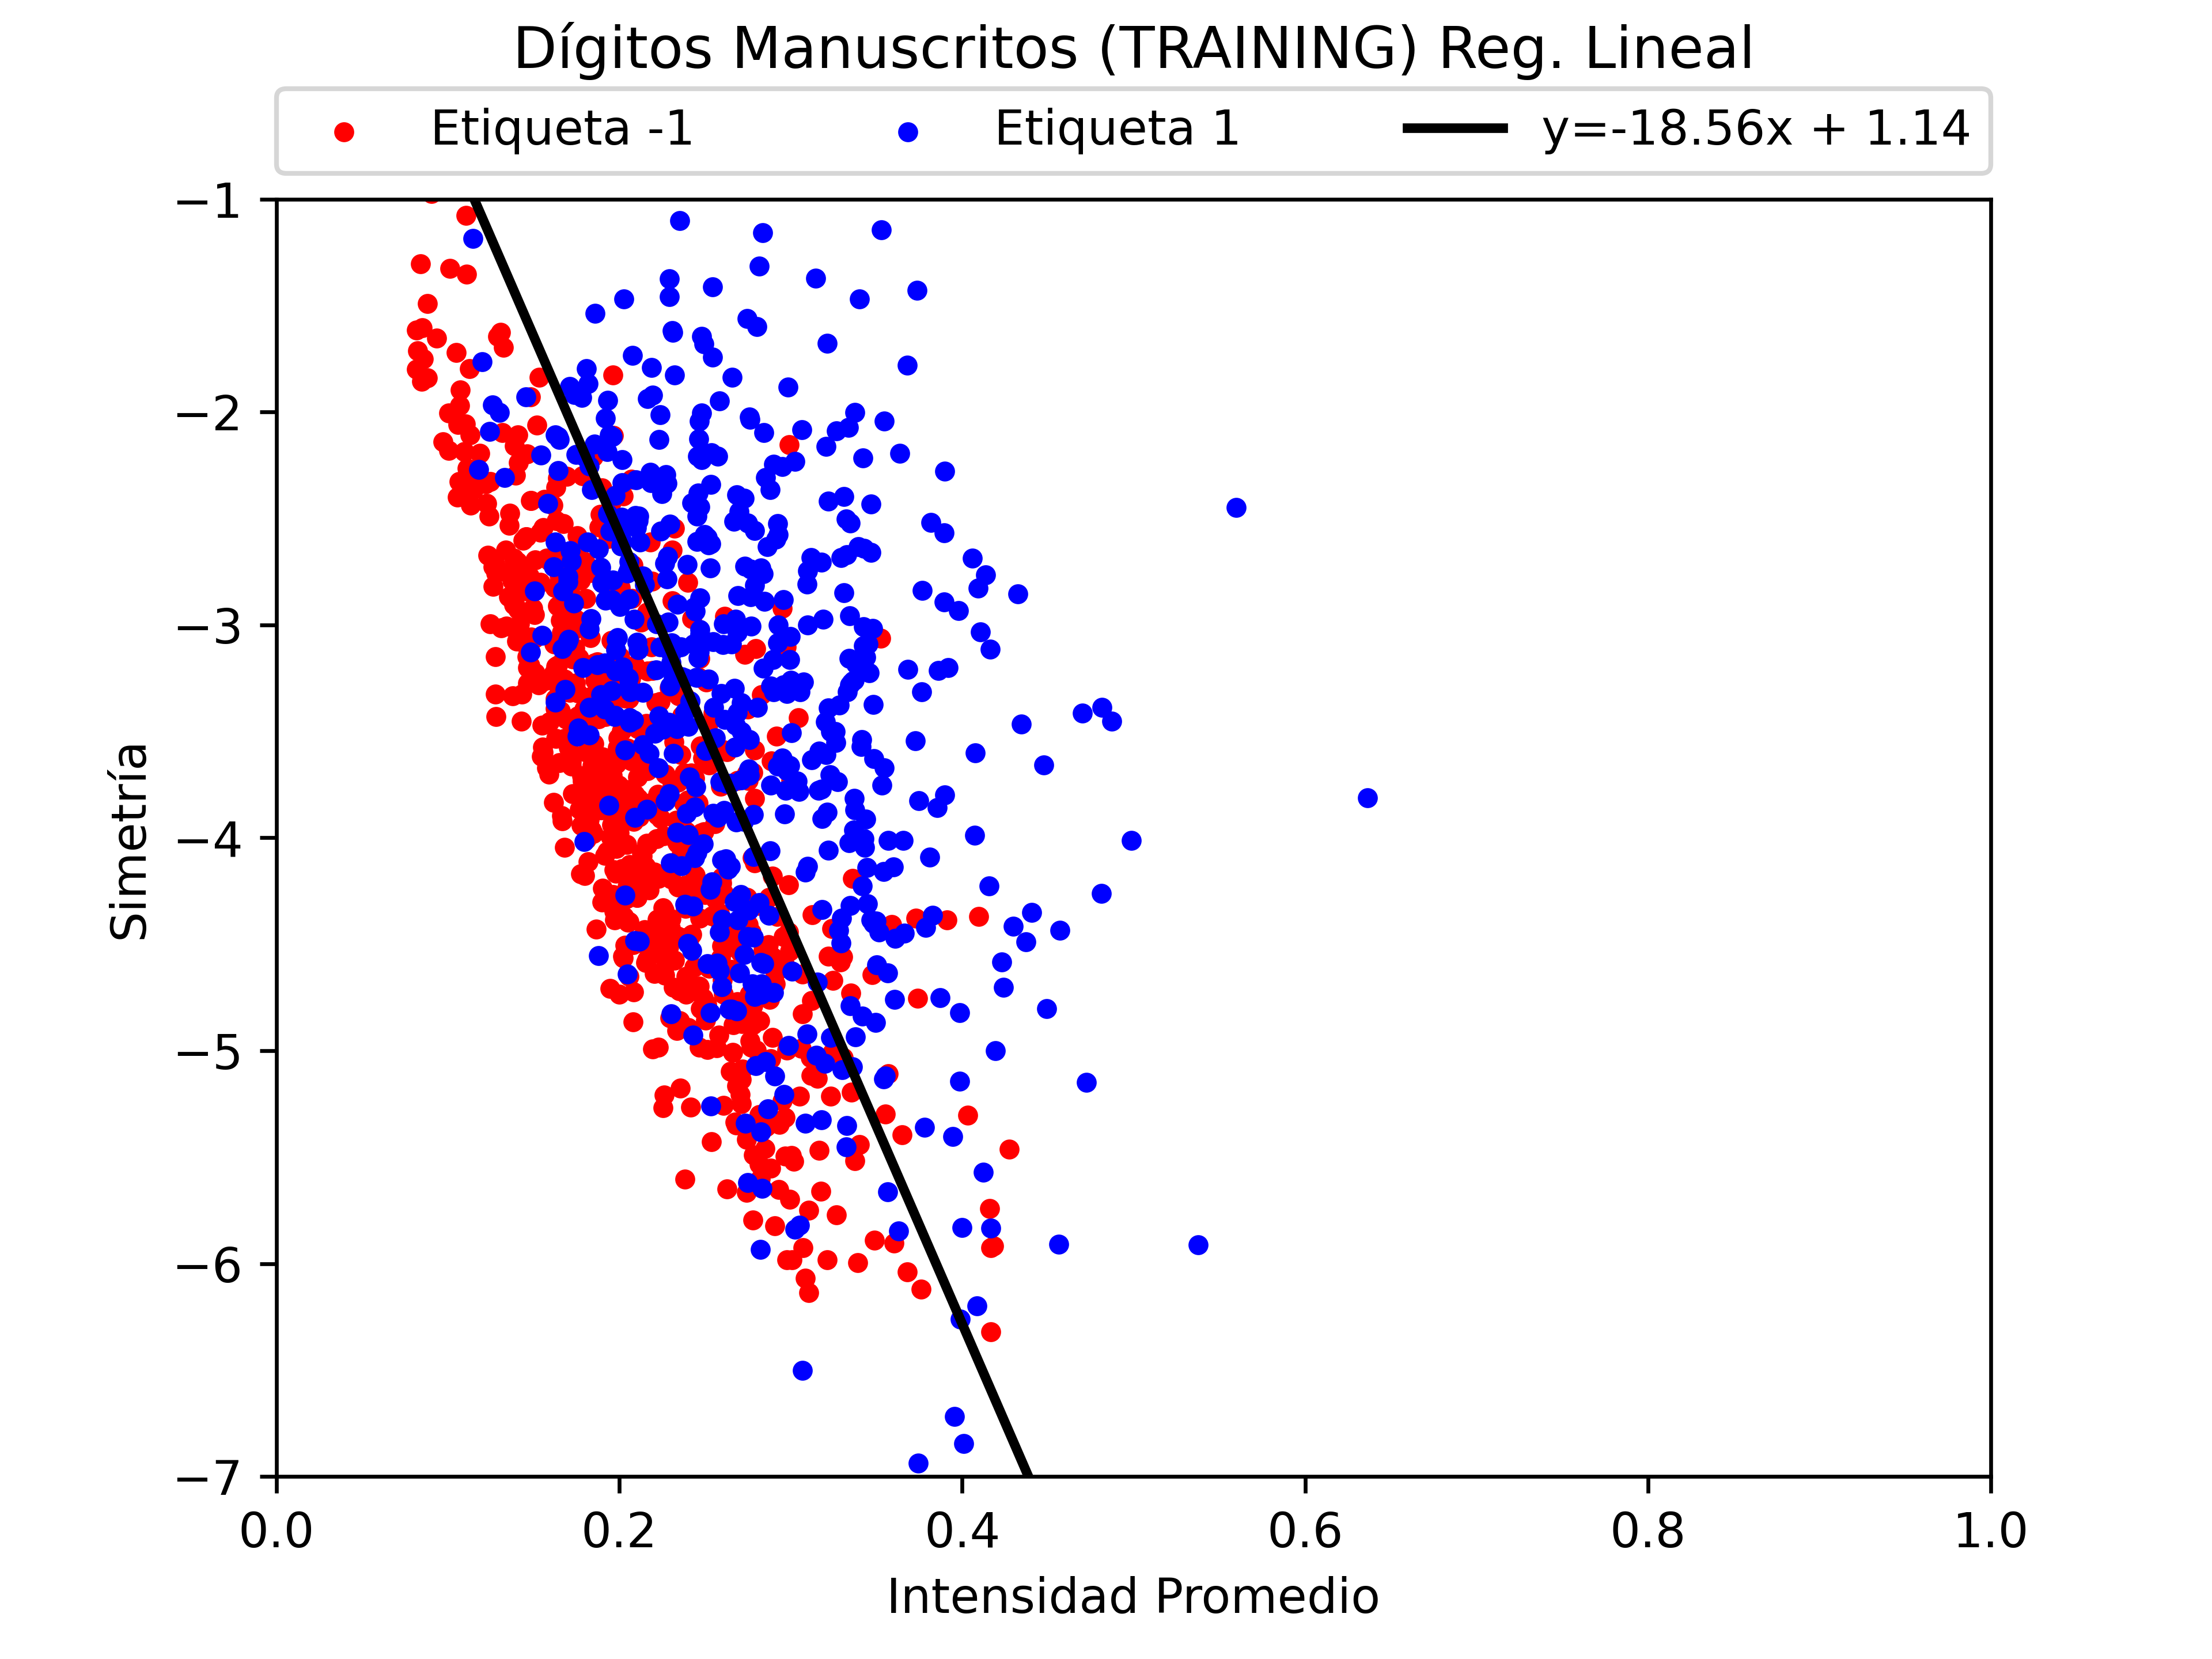
\includegraphics[width=0.9\textwidth]{Figure_15}
      \subcaption{Datos de entrenamiento} \label{subfig-5:dummy62}
    \end{minipage}
    \hfill \hfill
    \begin{minipage}[b]{.5\linewidth}
      \centering
      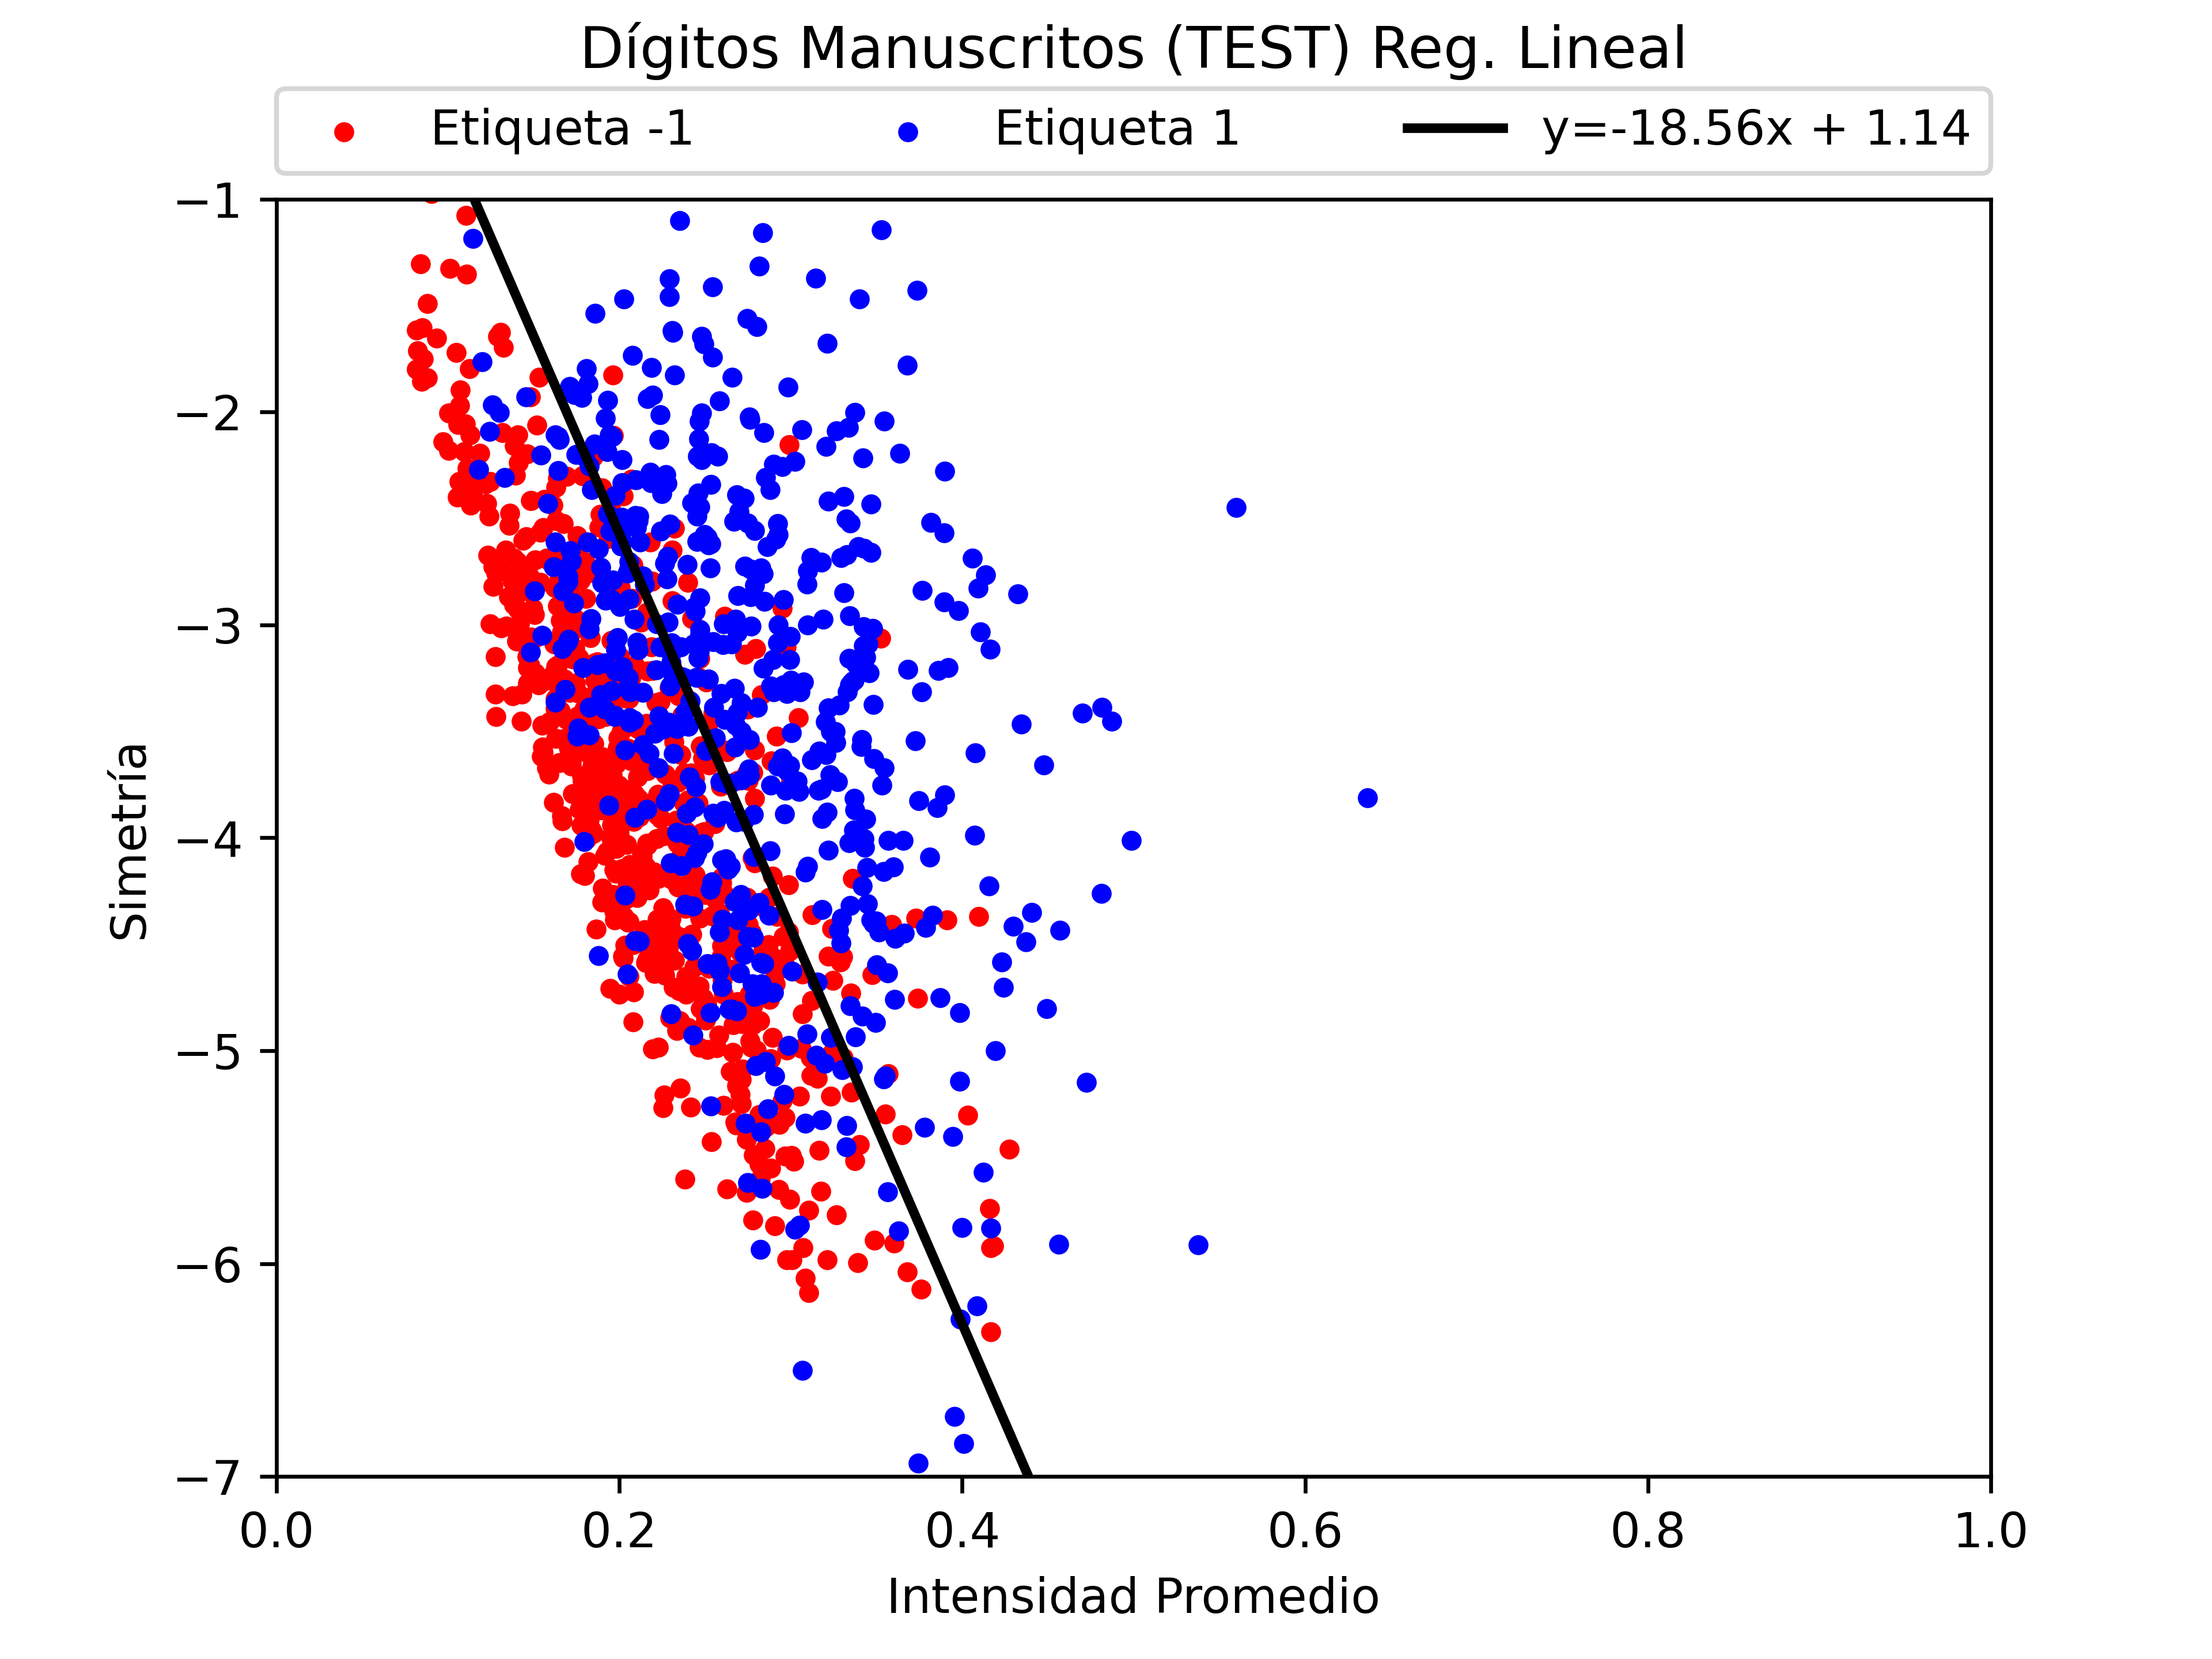
\includegraphics[width=0.9\textwidth]{Figure_16}
      \subcaption{Datos de test}
    \end{minipage}
    \label{fig:dummy62}
\end{figure}

\begin{figure}[H]
    \caption{PLA - Algoritmo de aprendizaje del perceptrón\medskip}
    \begin{minipage}[b]{.5\linewidth}
      \centering
      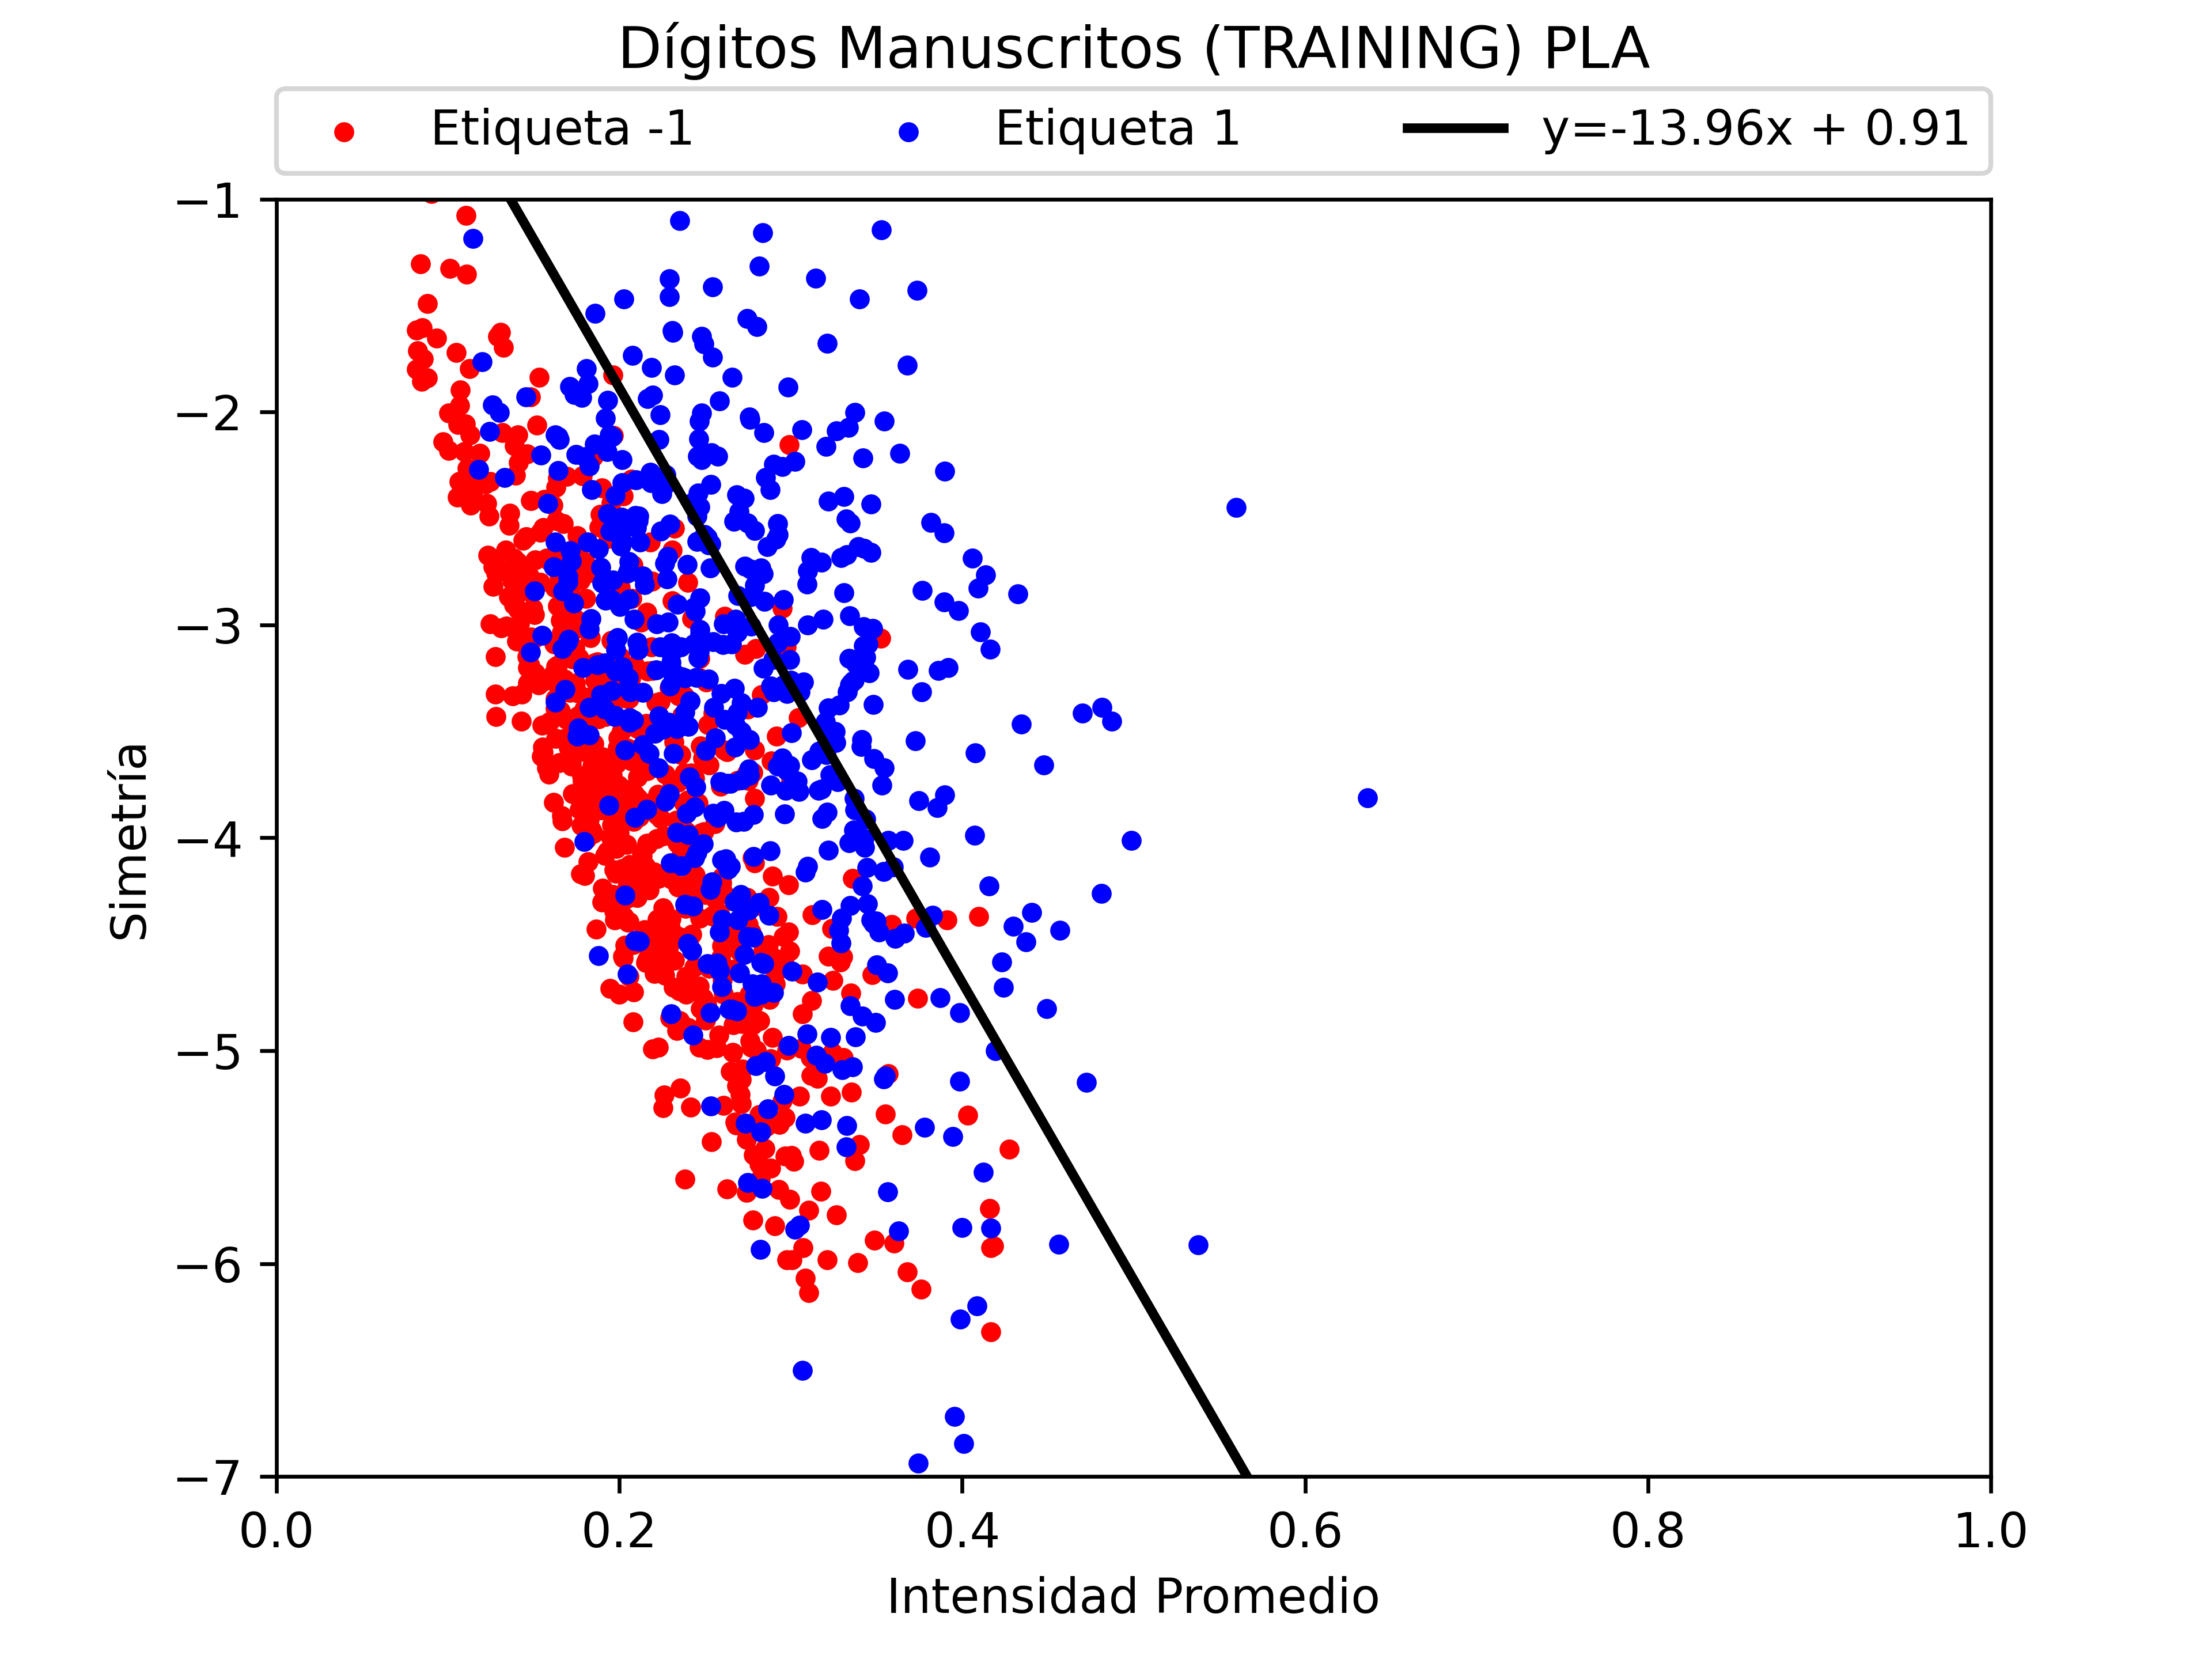
\includegraphics[width=0.9\textwidth]{Figure_17}
      \subcaption{Datos de entrenamiento} \label{subfig-5:dummy63}
    \end{minipage}
    \hfill \hfill
    \begin{minipage}[b]{.5\linewidth}
      \centering
      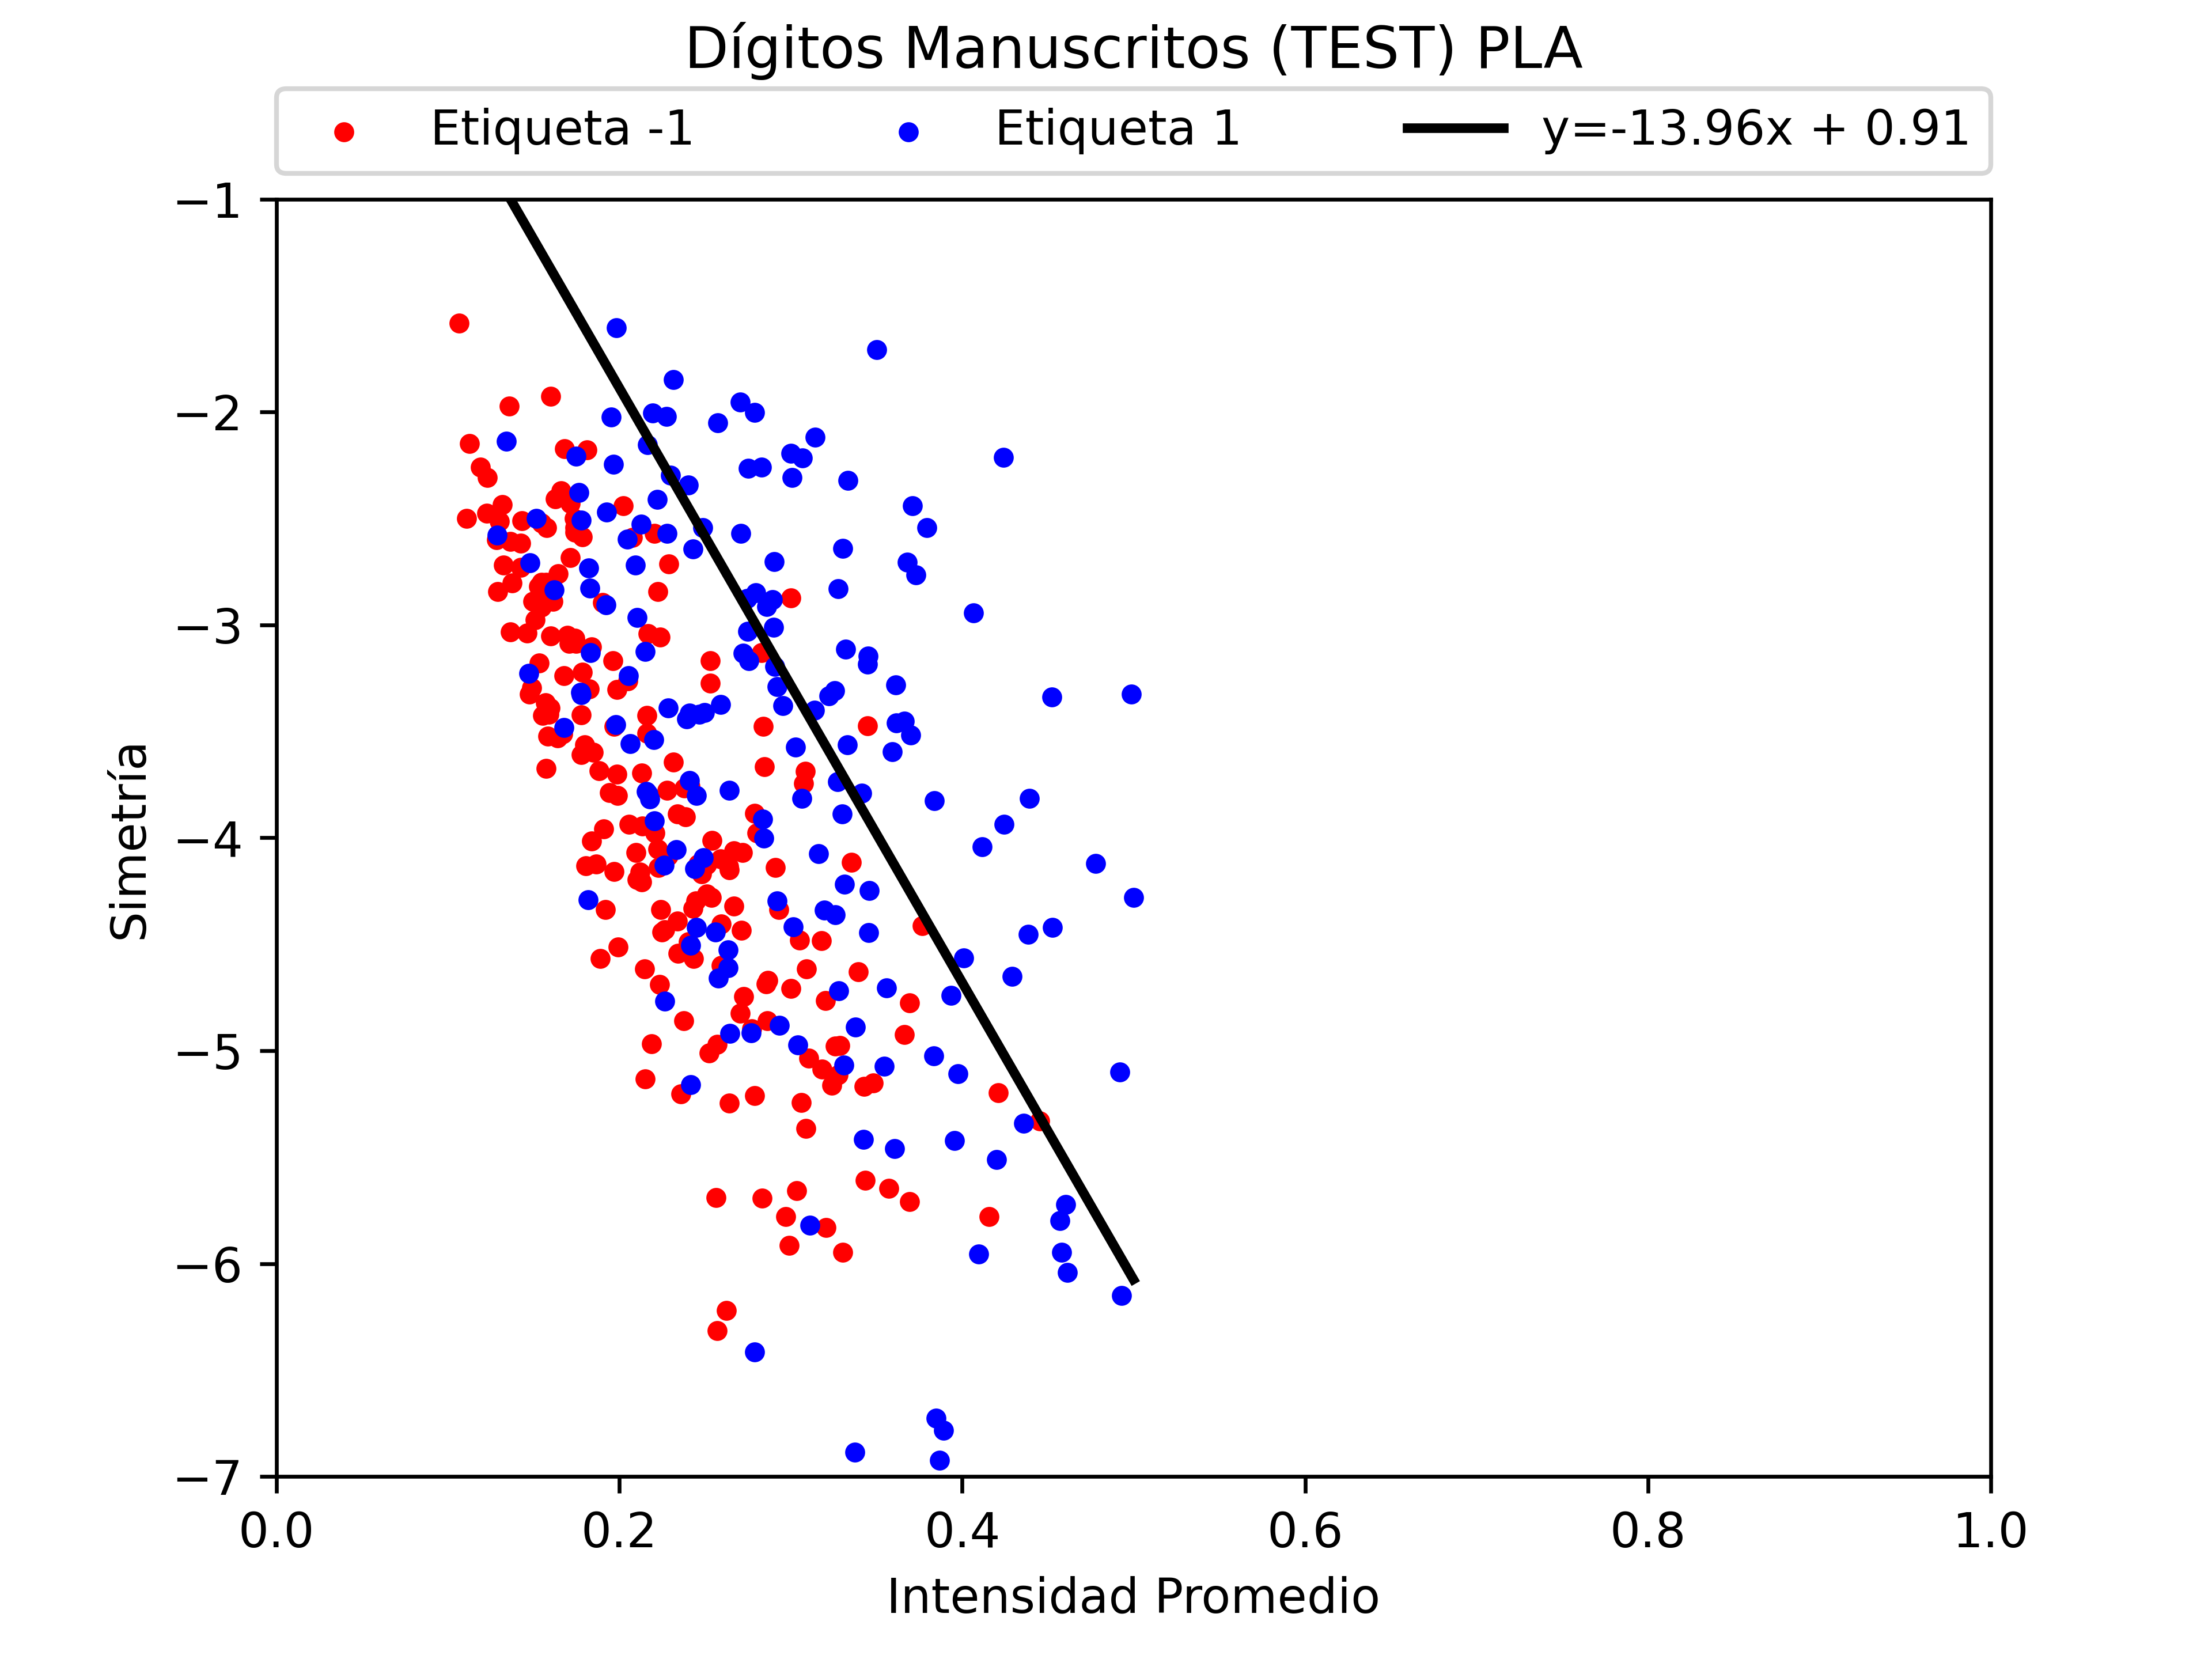
\includegraphics[width=0.9\textwidth]{Figure_18}
      \subcaption{Datos de test}
    \end{minipage}
    \label{fig:dummy63}
\end{figure}

\begin{figure}[H]
    \caption{RL - Regresión Logística para clasificación lineal\medskip}
    \begin{minipage}[b]{.5\linewidth}
      \centering
      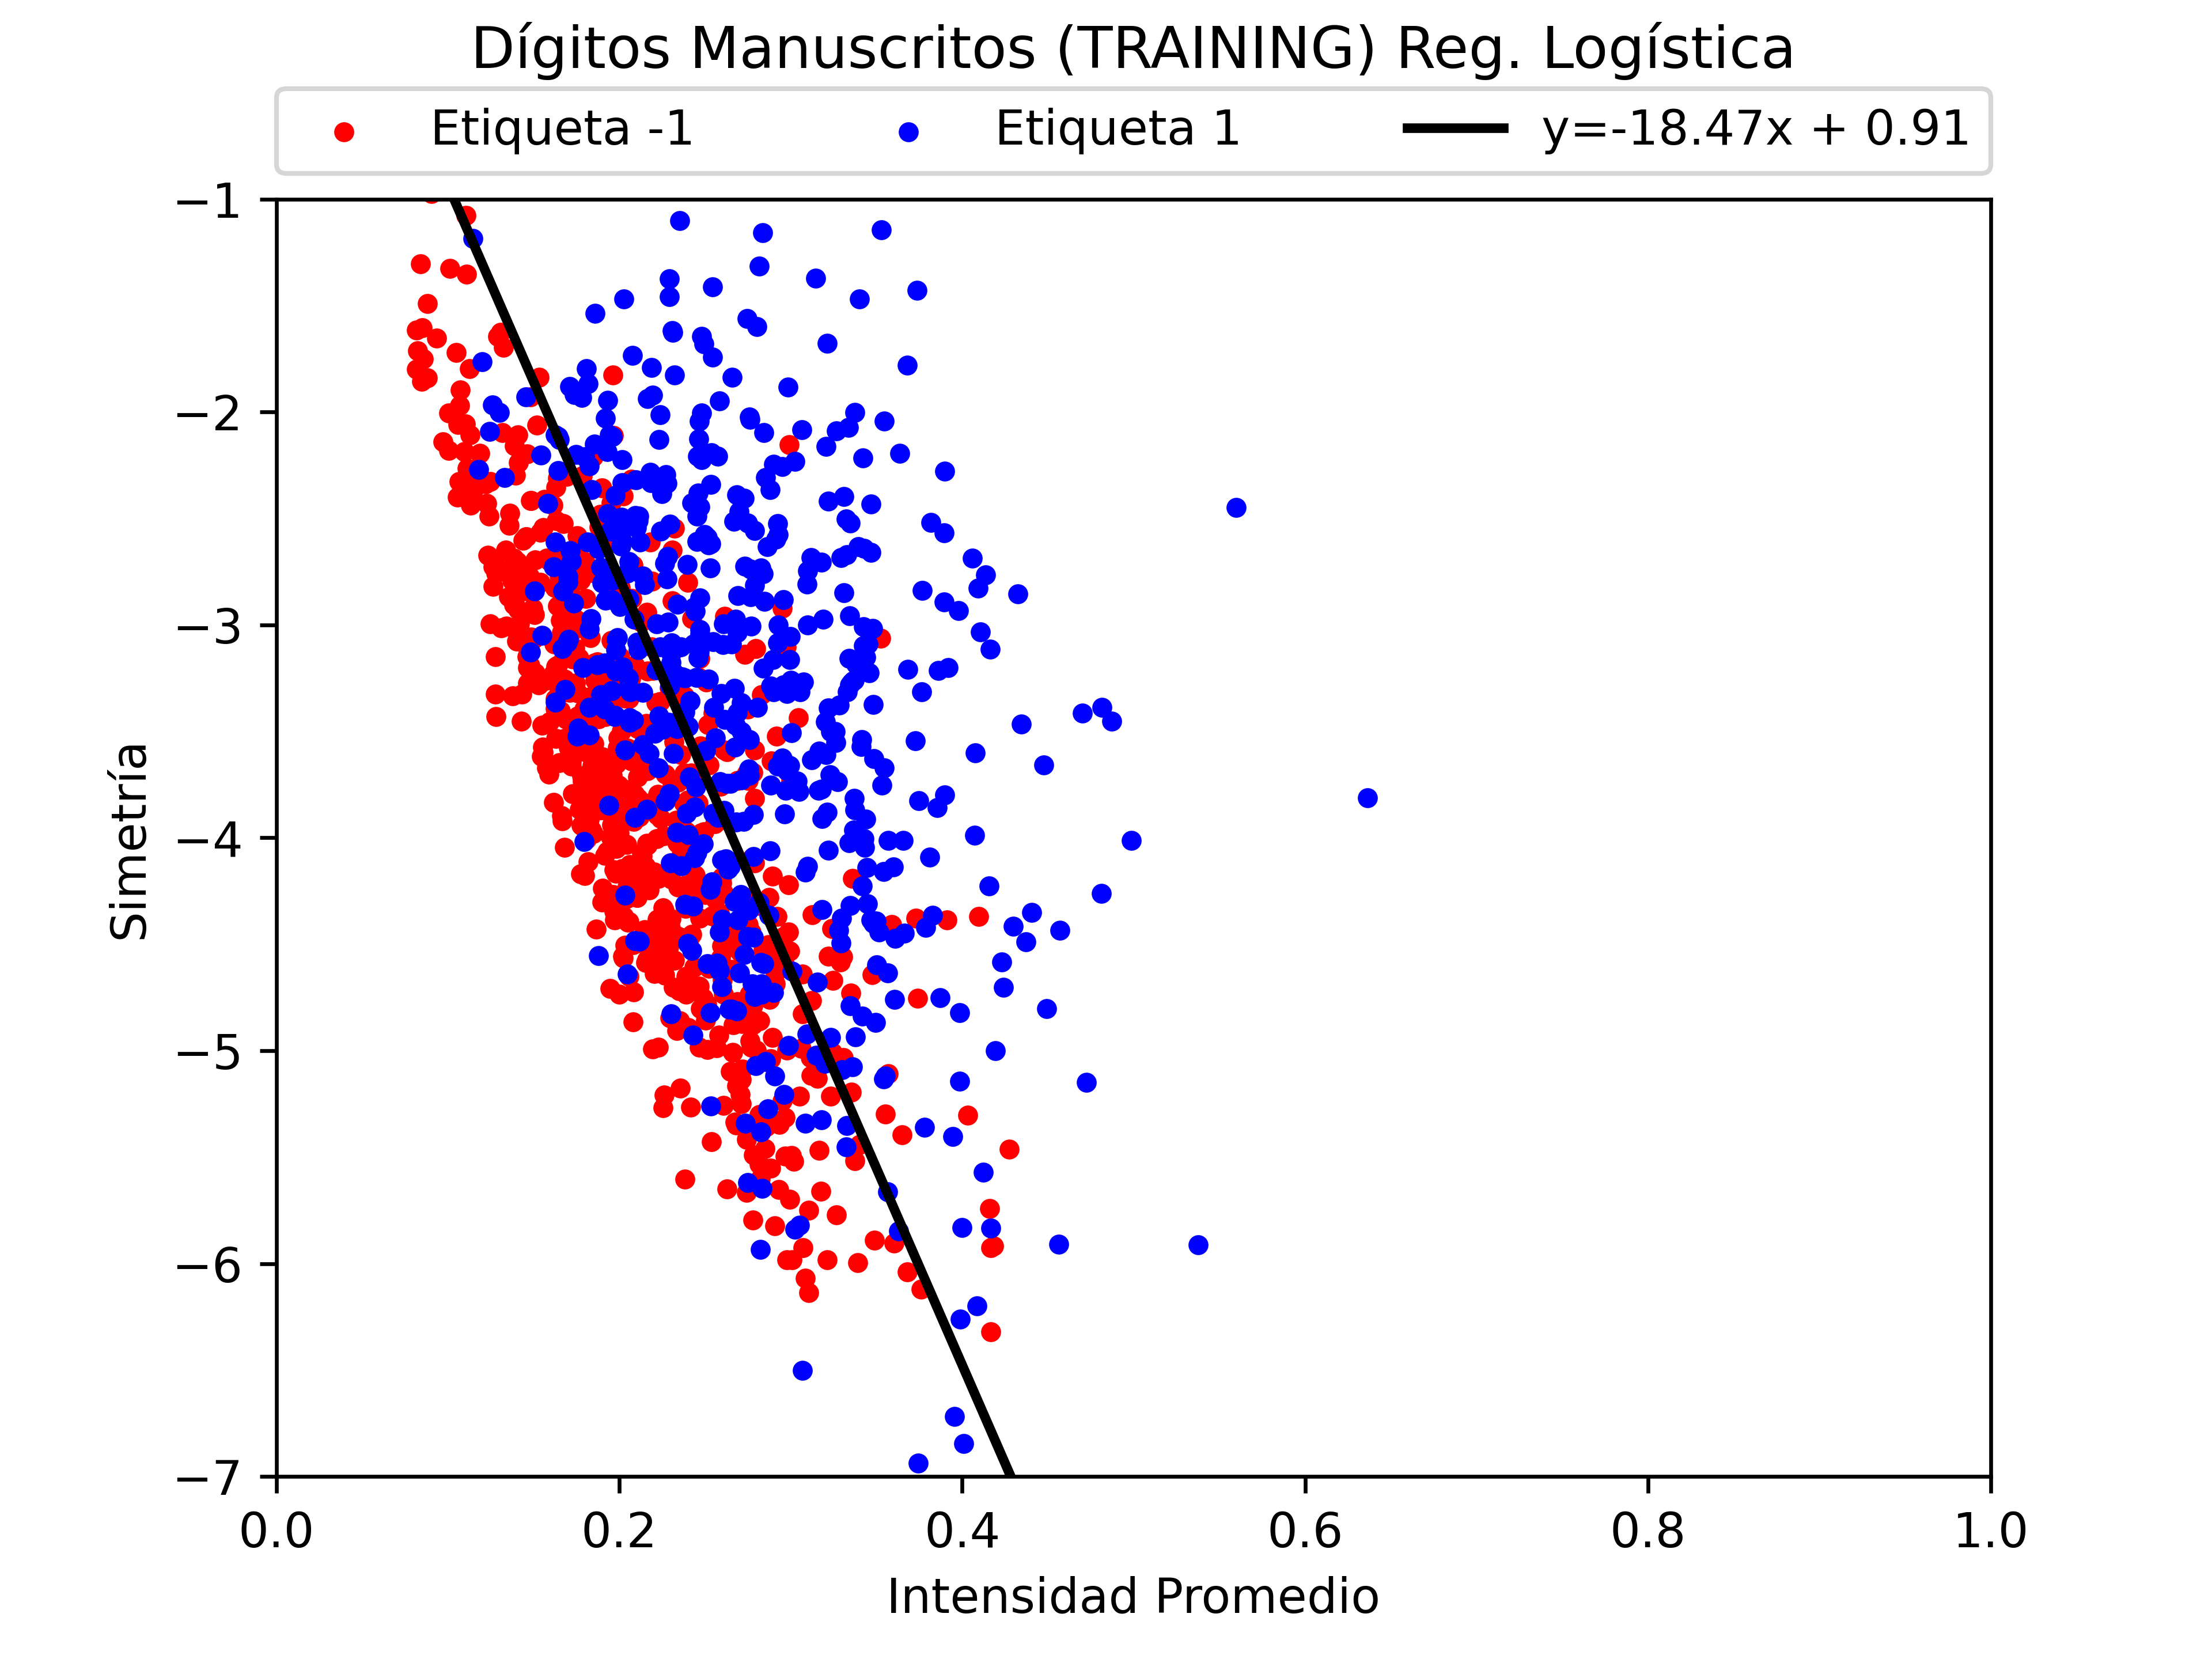
\includegraphics[width=0.9\textwidth]{Figure_19}
      \subcaption{Datos de entrenamiento} \label{subfig-5:dummy64}
    \end{minipage}
    \hfill \hfill
    \begin{minipage}[b]{.5\linewidth}
      \centering
      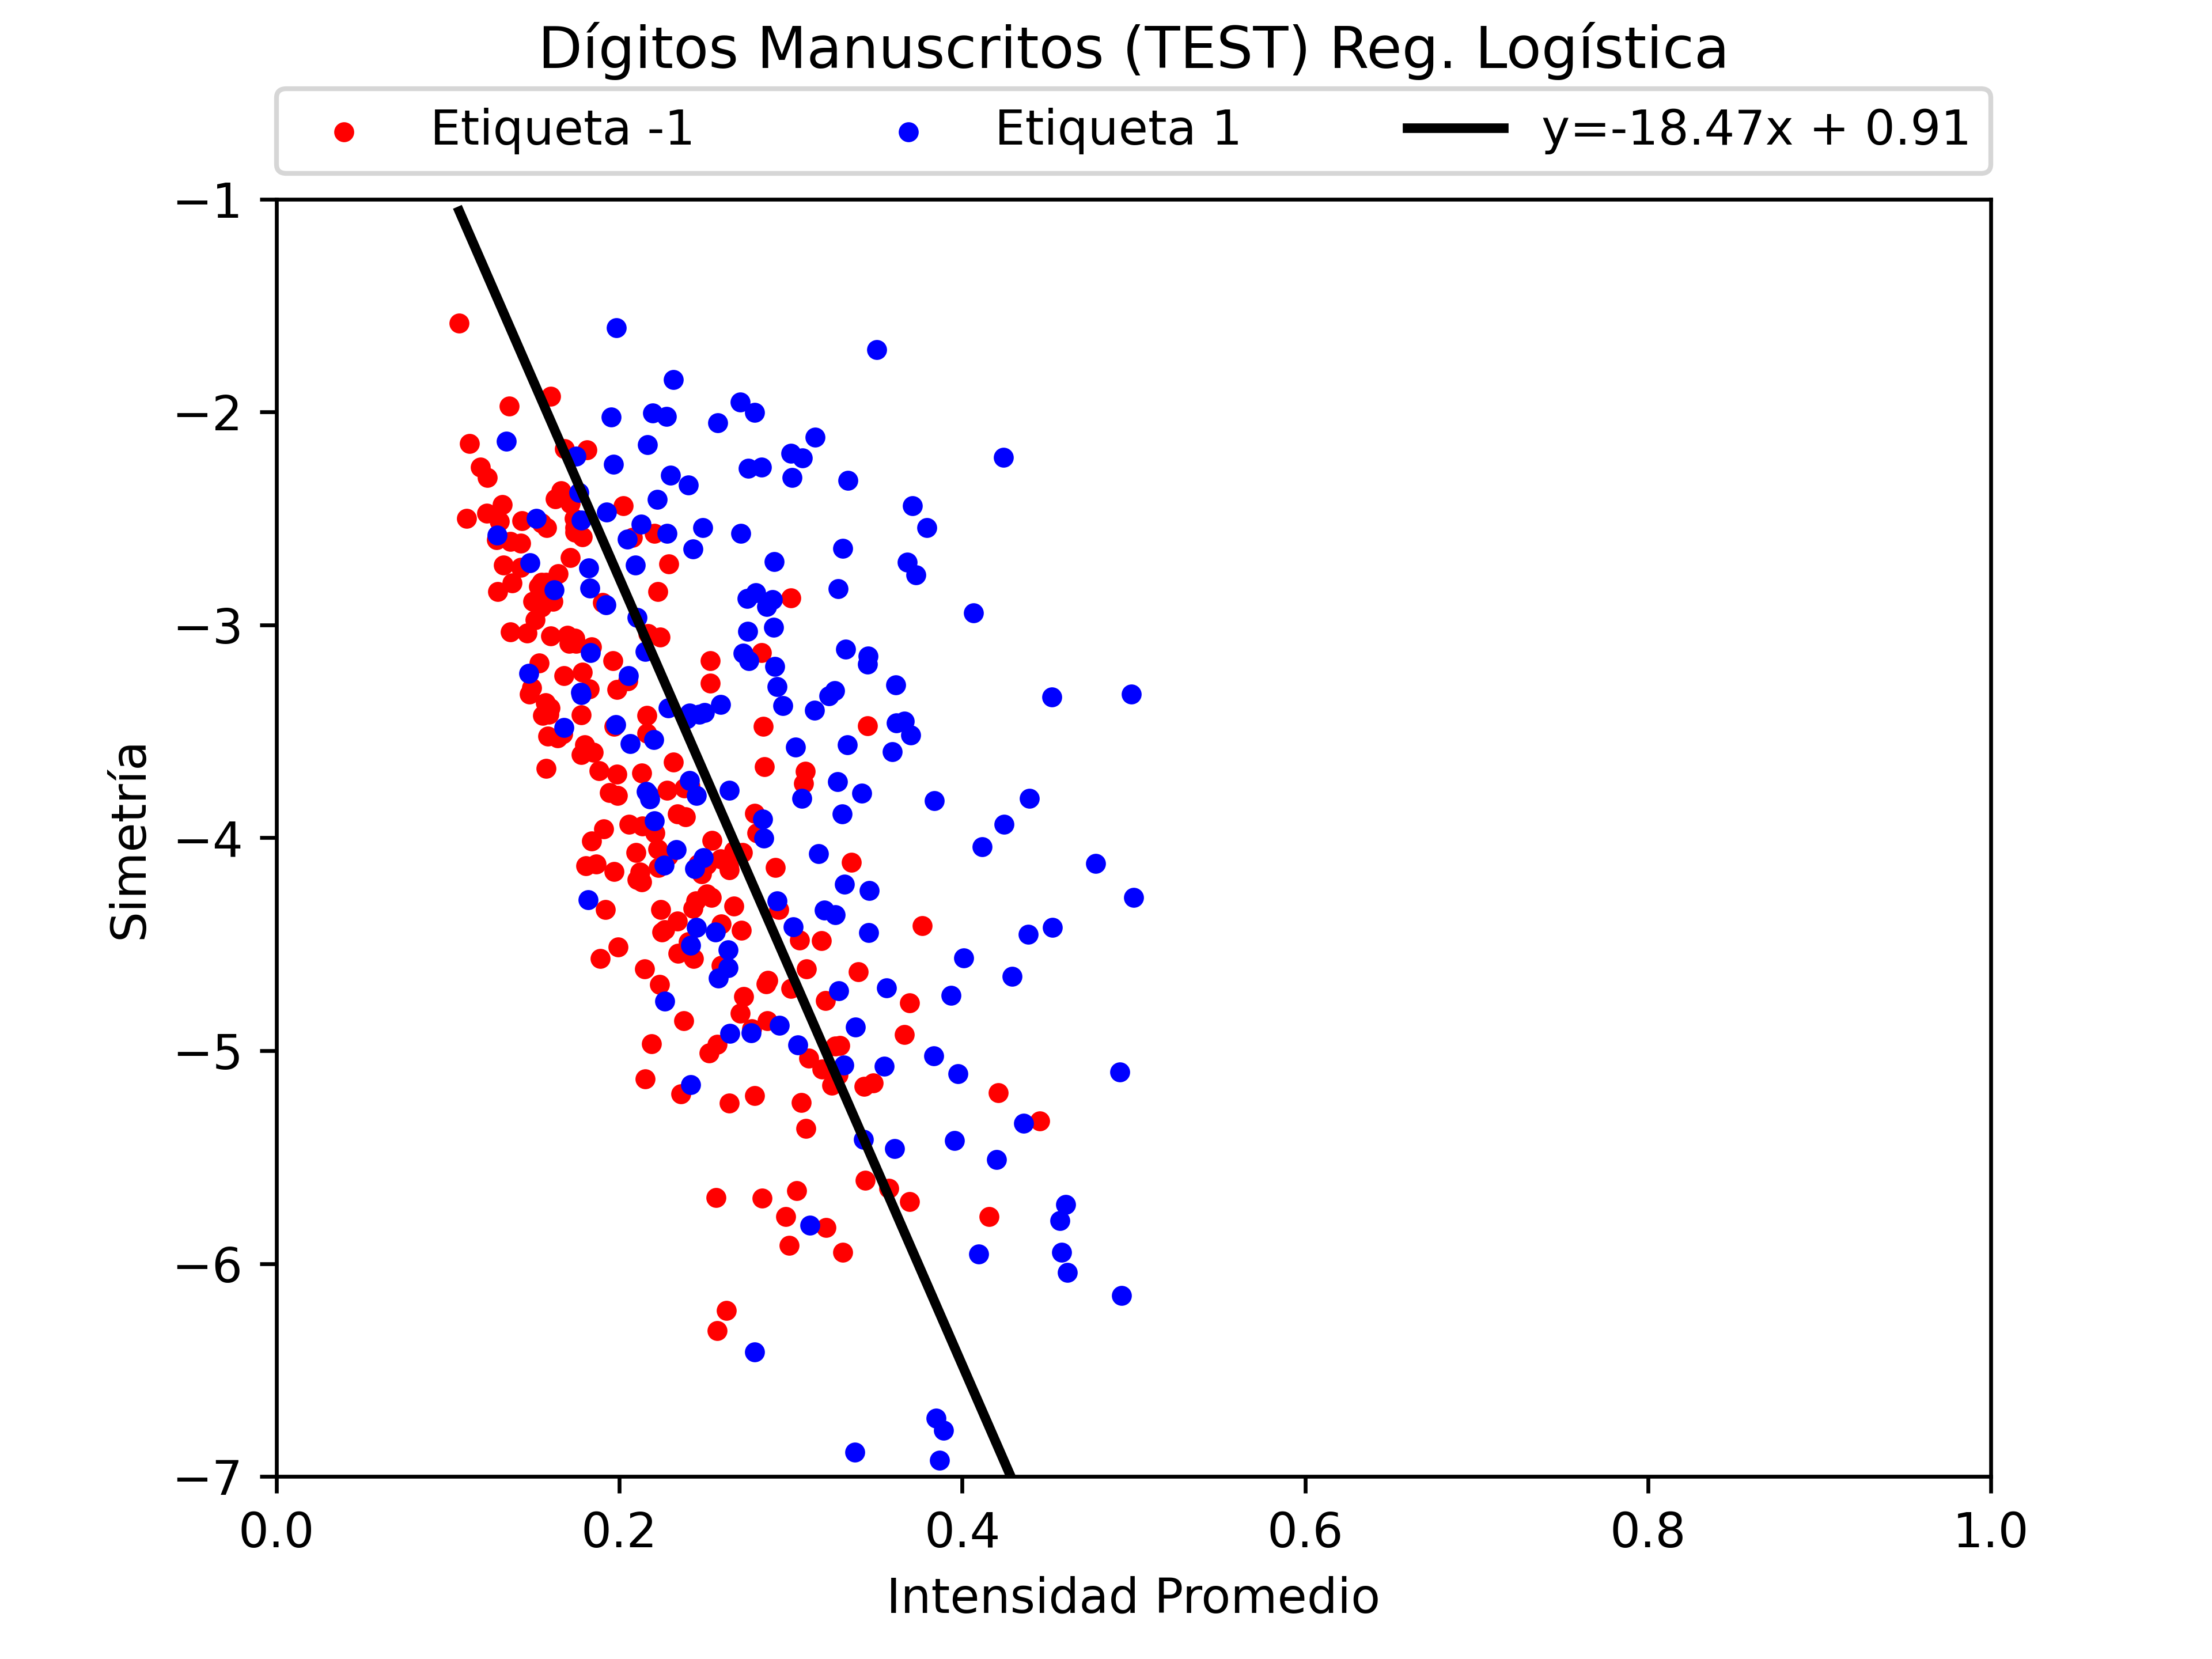
\includegraphics[width=0.9\textwidth]{Figure_20}
      \subcaption{Datos de test}
    \end{minipage}
    \label{fig:dummy64}
\end{figure}

\begin{figure}[H]
    \caption{Algoritmo PLA-POCKET \medskip}
    \begin{minipage}[b]{.5\linewidth}
      \centering
      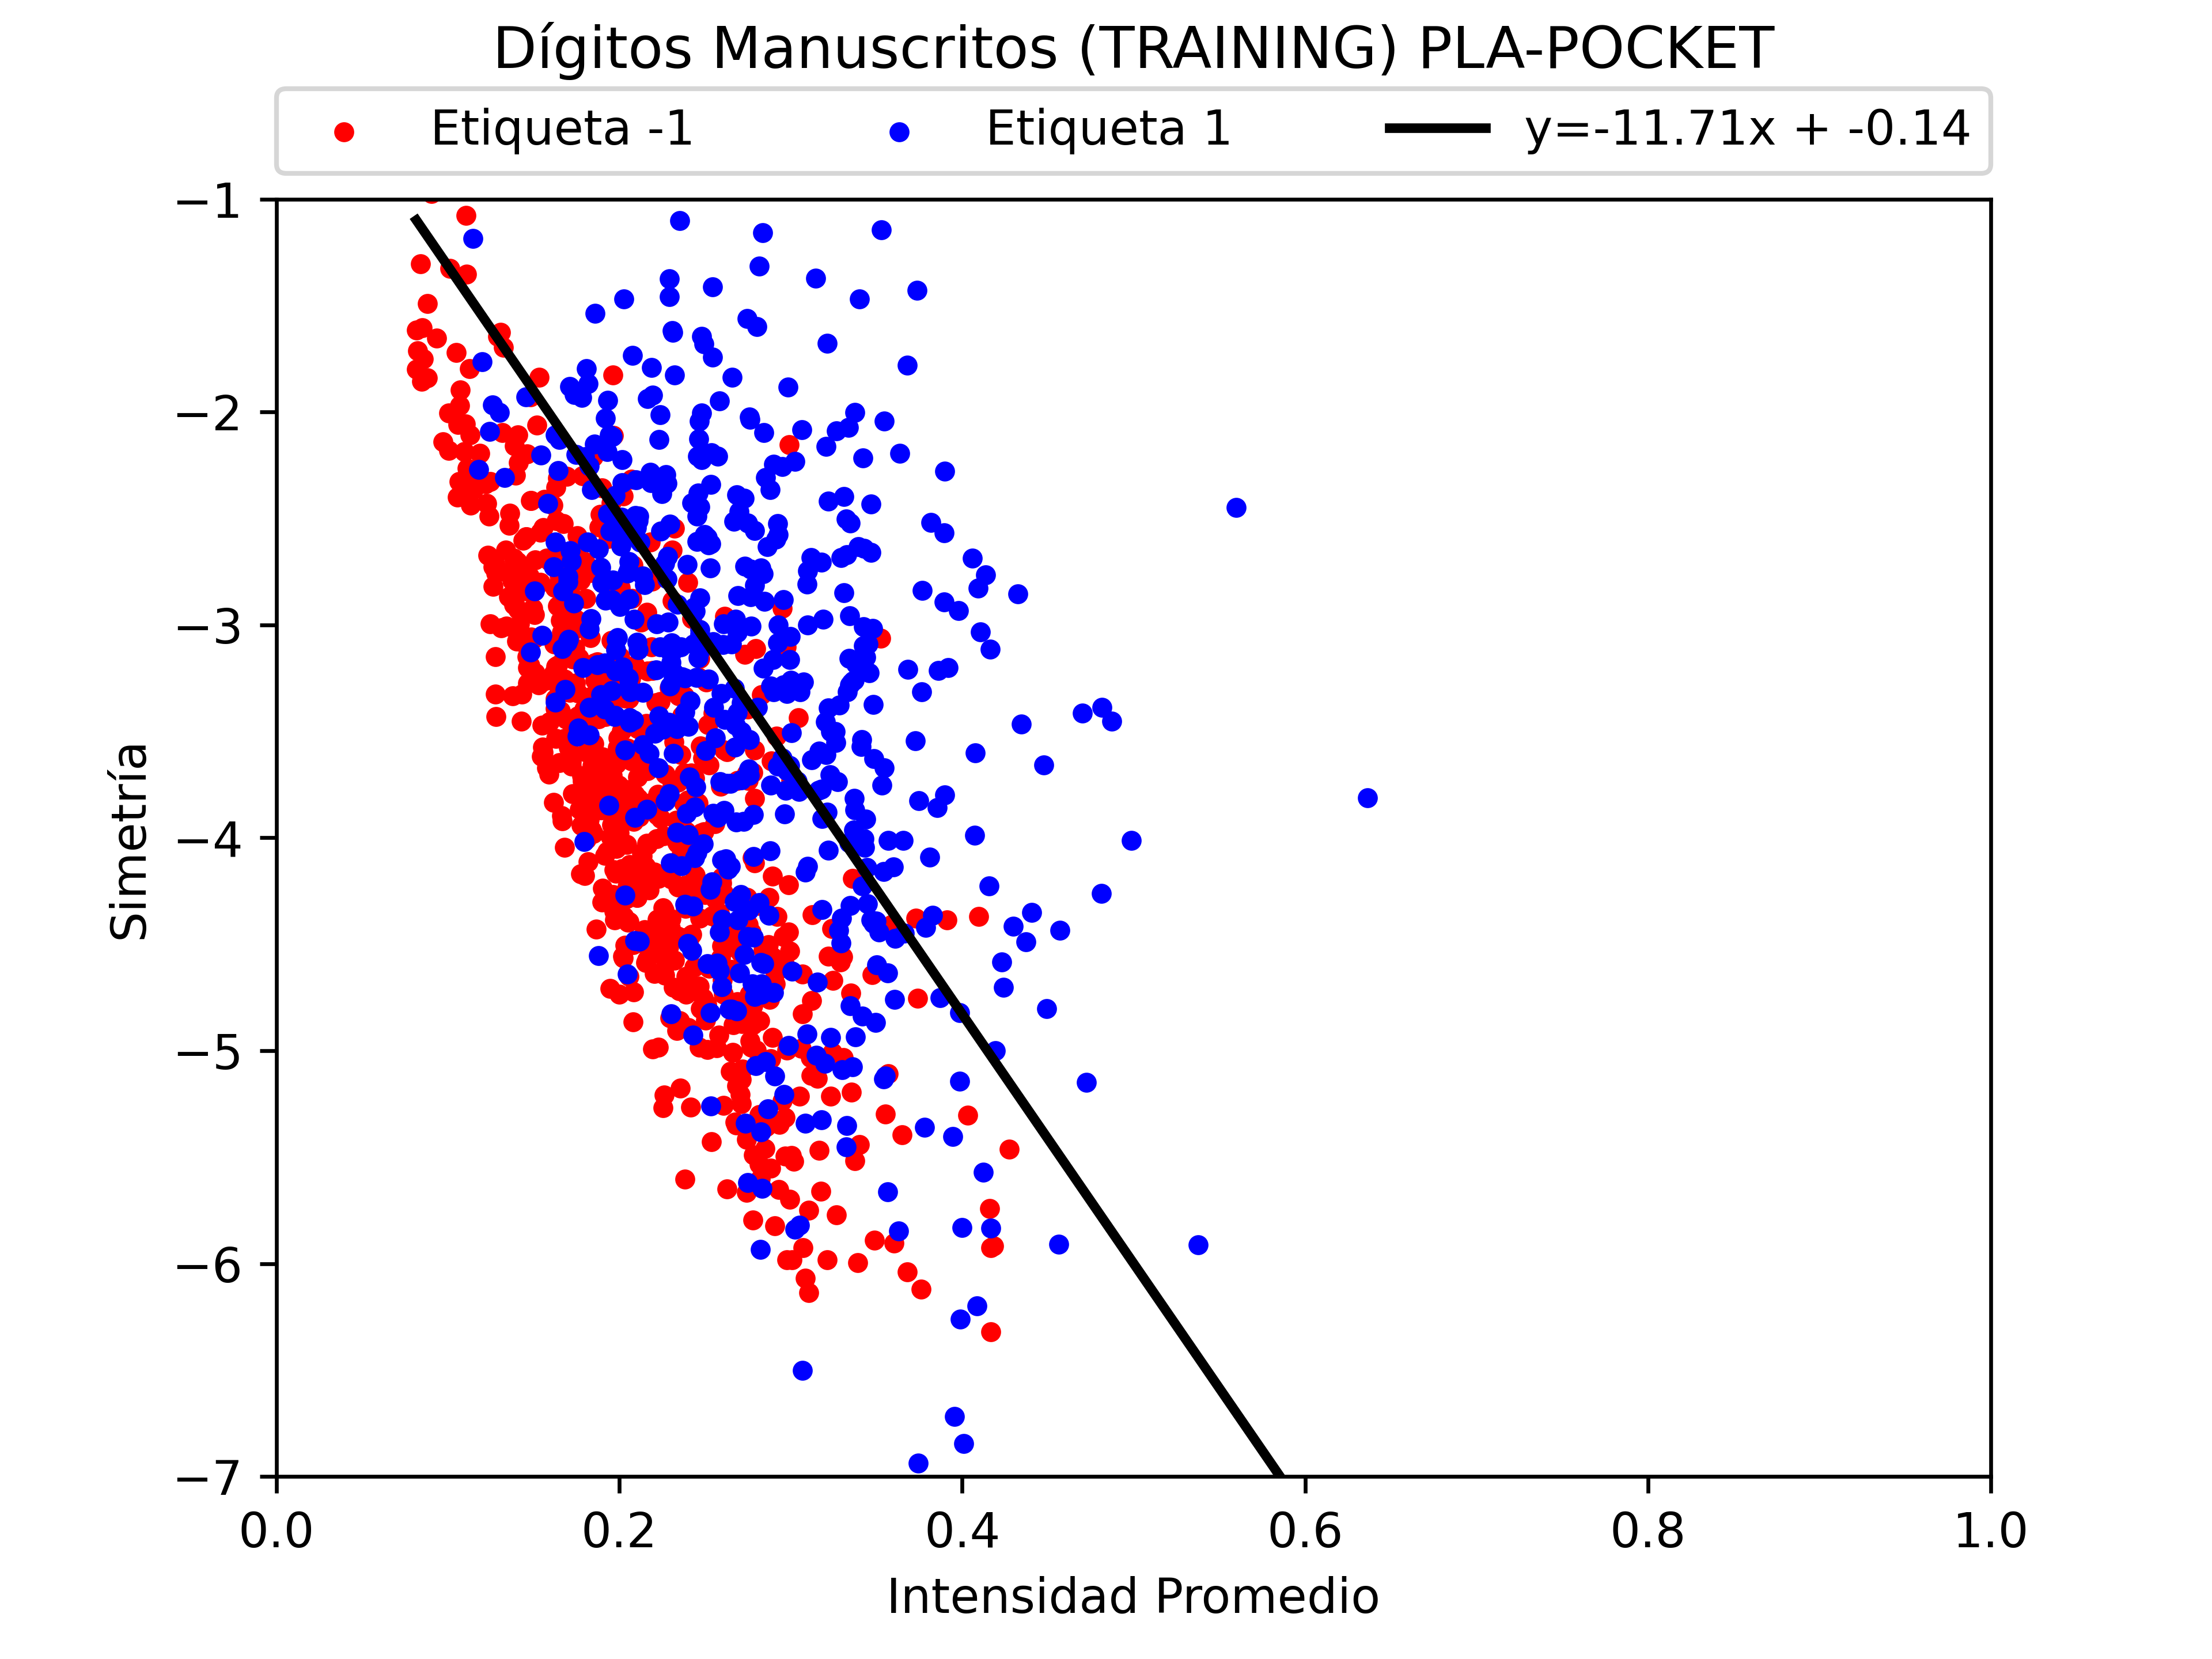
\includegraphics[width=0.9\textwidth]{Figure_21}
      \subcaption{Datos de entrenamiento} \label{subfig-5:dummy65}
    \end{minipage}
    \hfill \hfill
    \begin{minipage}[b]{.5\linewidth}
      \centering
      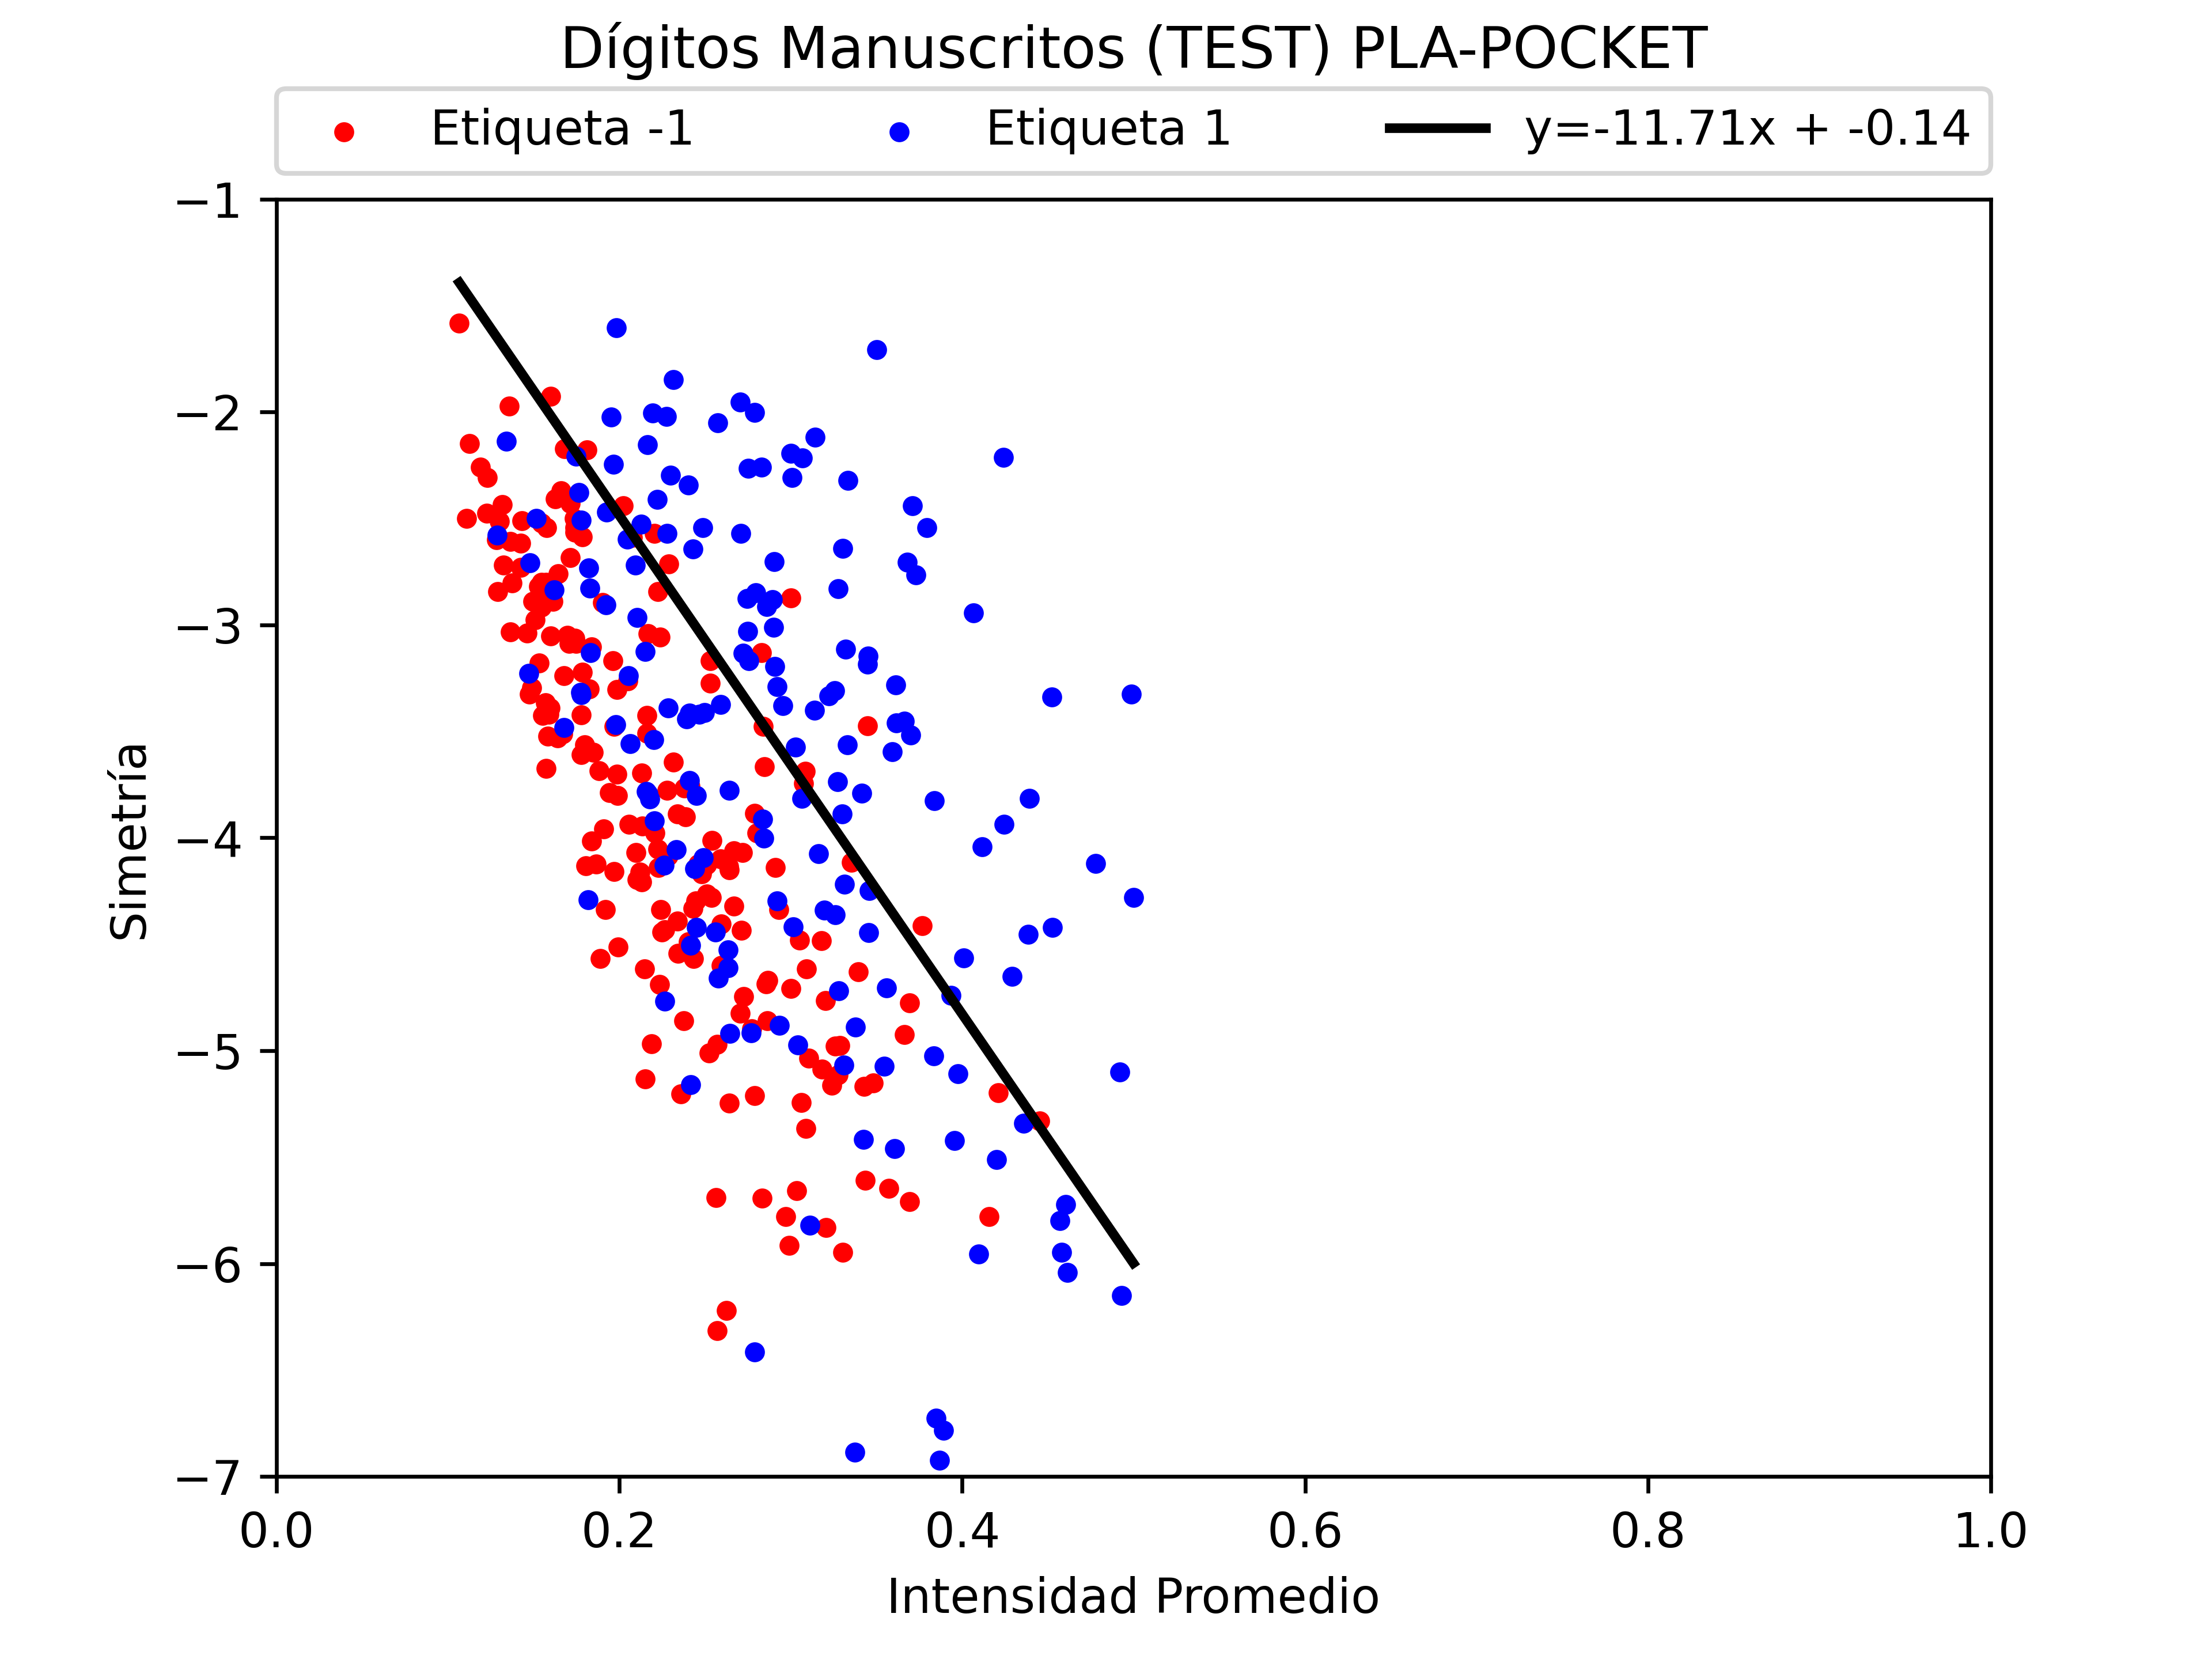
\includegraphics[width=0.9\textwidth]{Figure_22}
      \subcaption{Datos de test}
    \end{minipage}
    \label{fig:dummy65}
\end{figure}

\subsection{Calcular $E_{in}$ y $E_{test}$}

\begin{table}[H]
    \centering
    \begin{tabular}{llll} \toprule
        Algoritmo & $E_{in}$ & $E_{test}$ & Iteraciones \\ \midrule
        Regresión Lineal& $0.643$ & $0.709$ & ----- \\ 
        PLA & $0.309$ & $0.301$ & $1000$ \\ 
        Regresión Logística & $0.464$ & $0.526$ & $571$ \\ 
        PLA-POCKET & $0.220$ & $0.240$ & $8$ \\ \bottomrule
    \end{tabular}
    \caption{Comparación de los modelos lineales estudiados}
\end{table}

\subsection{Repetir inicialización con los pesos obtenidos mediante regresión lineal}

\textbf{Si se emplean los pesos obtenidos con regresión lineal para inicializar
los otros tres métodos (RL, PLA, PLA-pocket), ¿se observa alguna mejora en
los resultados a algún nivel? Justifique su respuesta}

Denominamos $w_{lin}$ a los pesos obtenidos tras aplicar regresión lineal al conjunto
de datos de entrenamiento.

\begin{figure}[H]
    \caption{PLA inicializado con $w_{lin}$ \medskip}
    \begin{minipage}[b]{.5\linewidth}
      \centering
      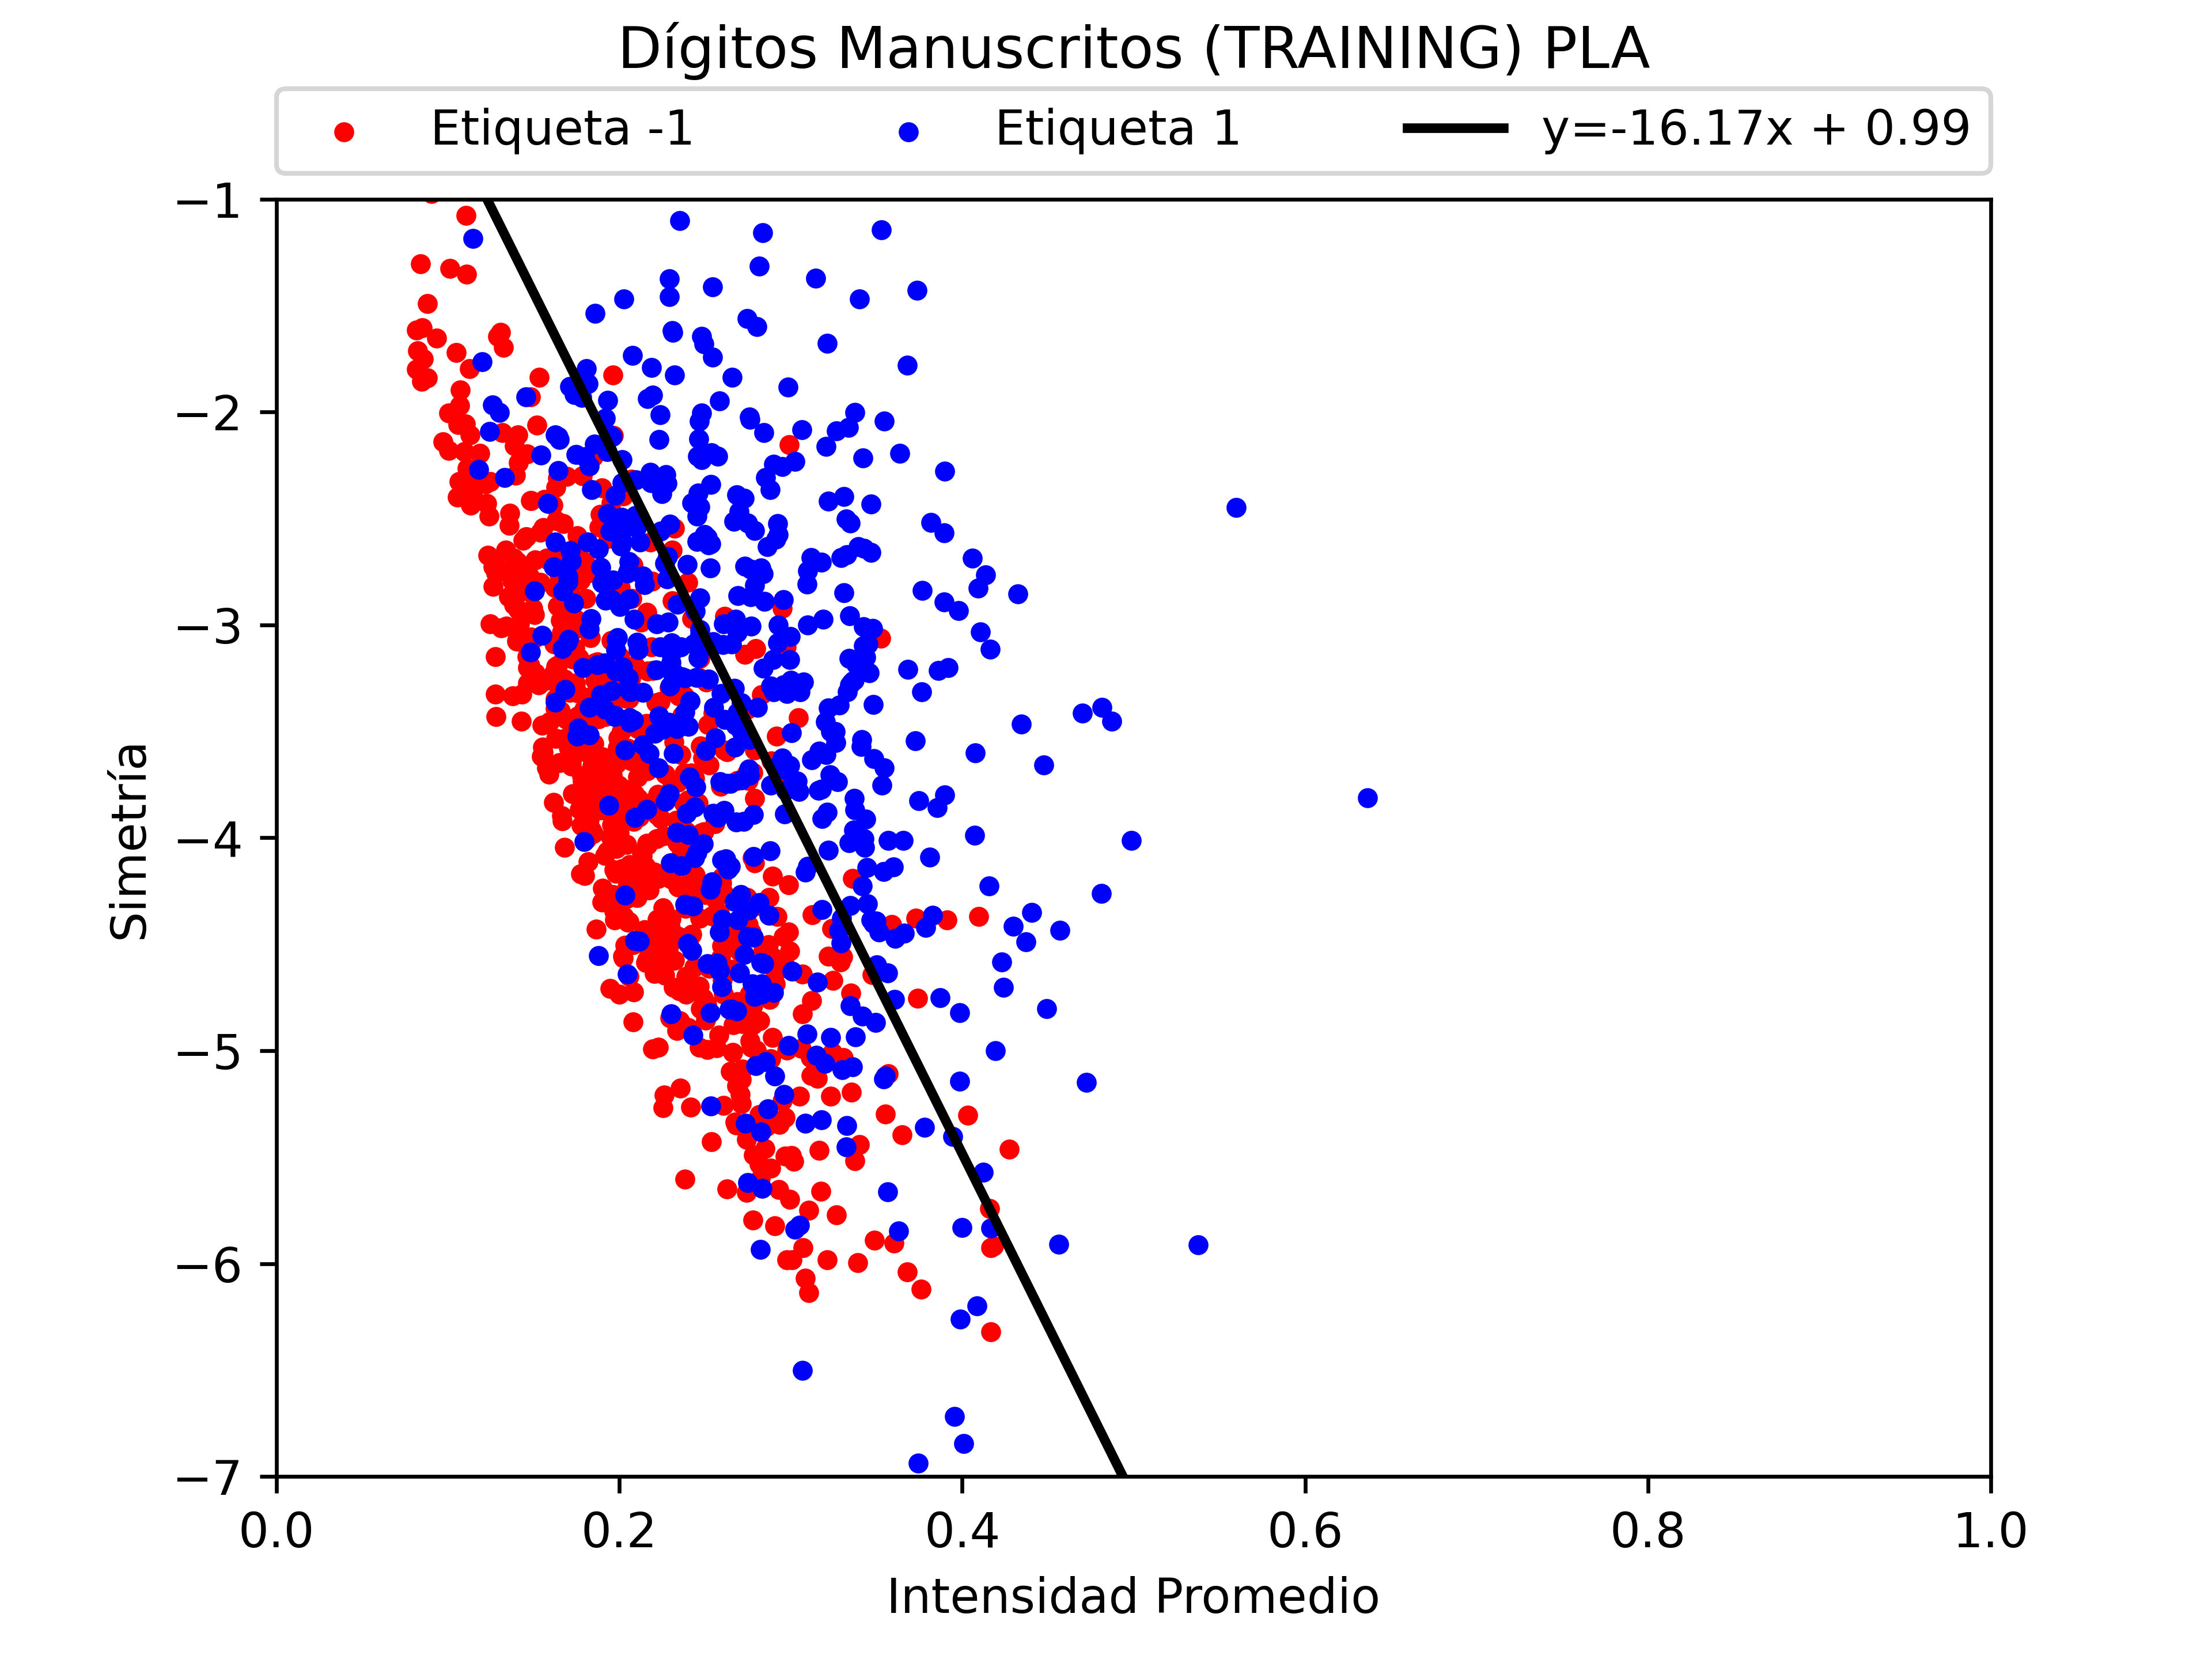
\includegraphics[width=0.9\textwidth]{Figure_23}
      \subcaption{Datos de entrenamiento} \label{subfig-5:dummy66}
    \end{minipage}
    \hfill \hfill
    \begin{minipage}[b]{.5\linewidth}
      \centering
      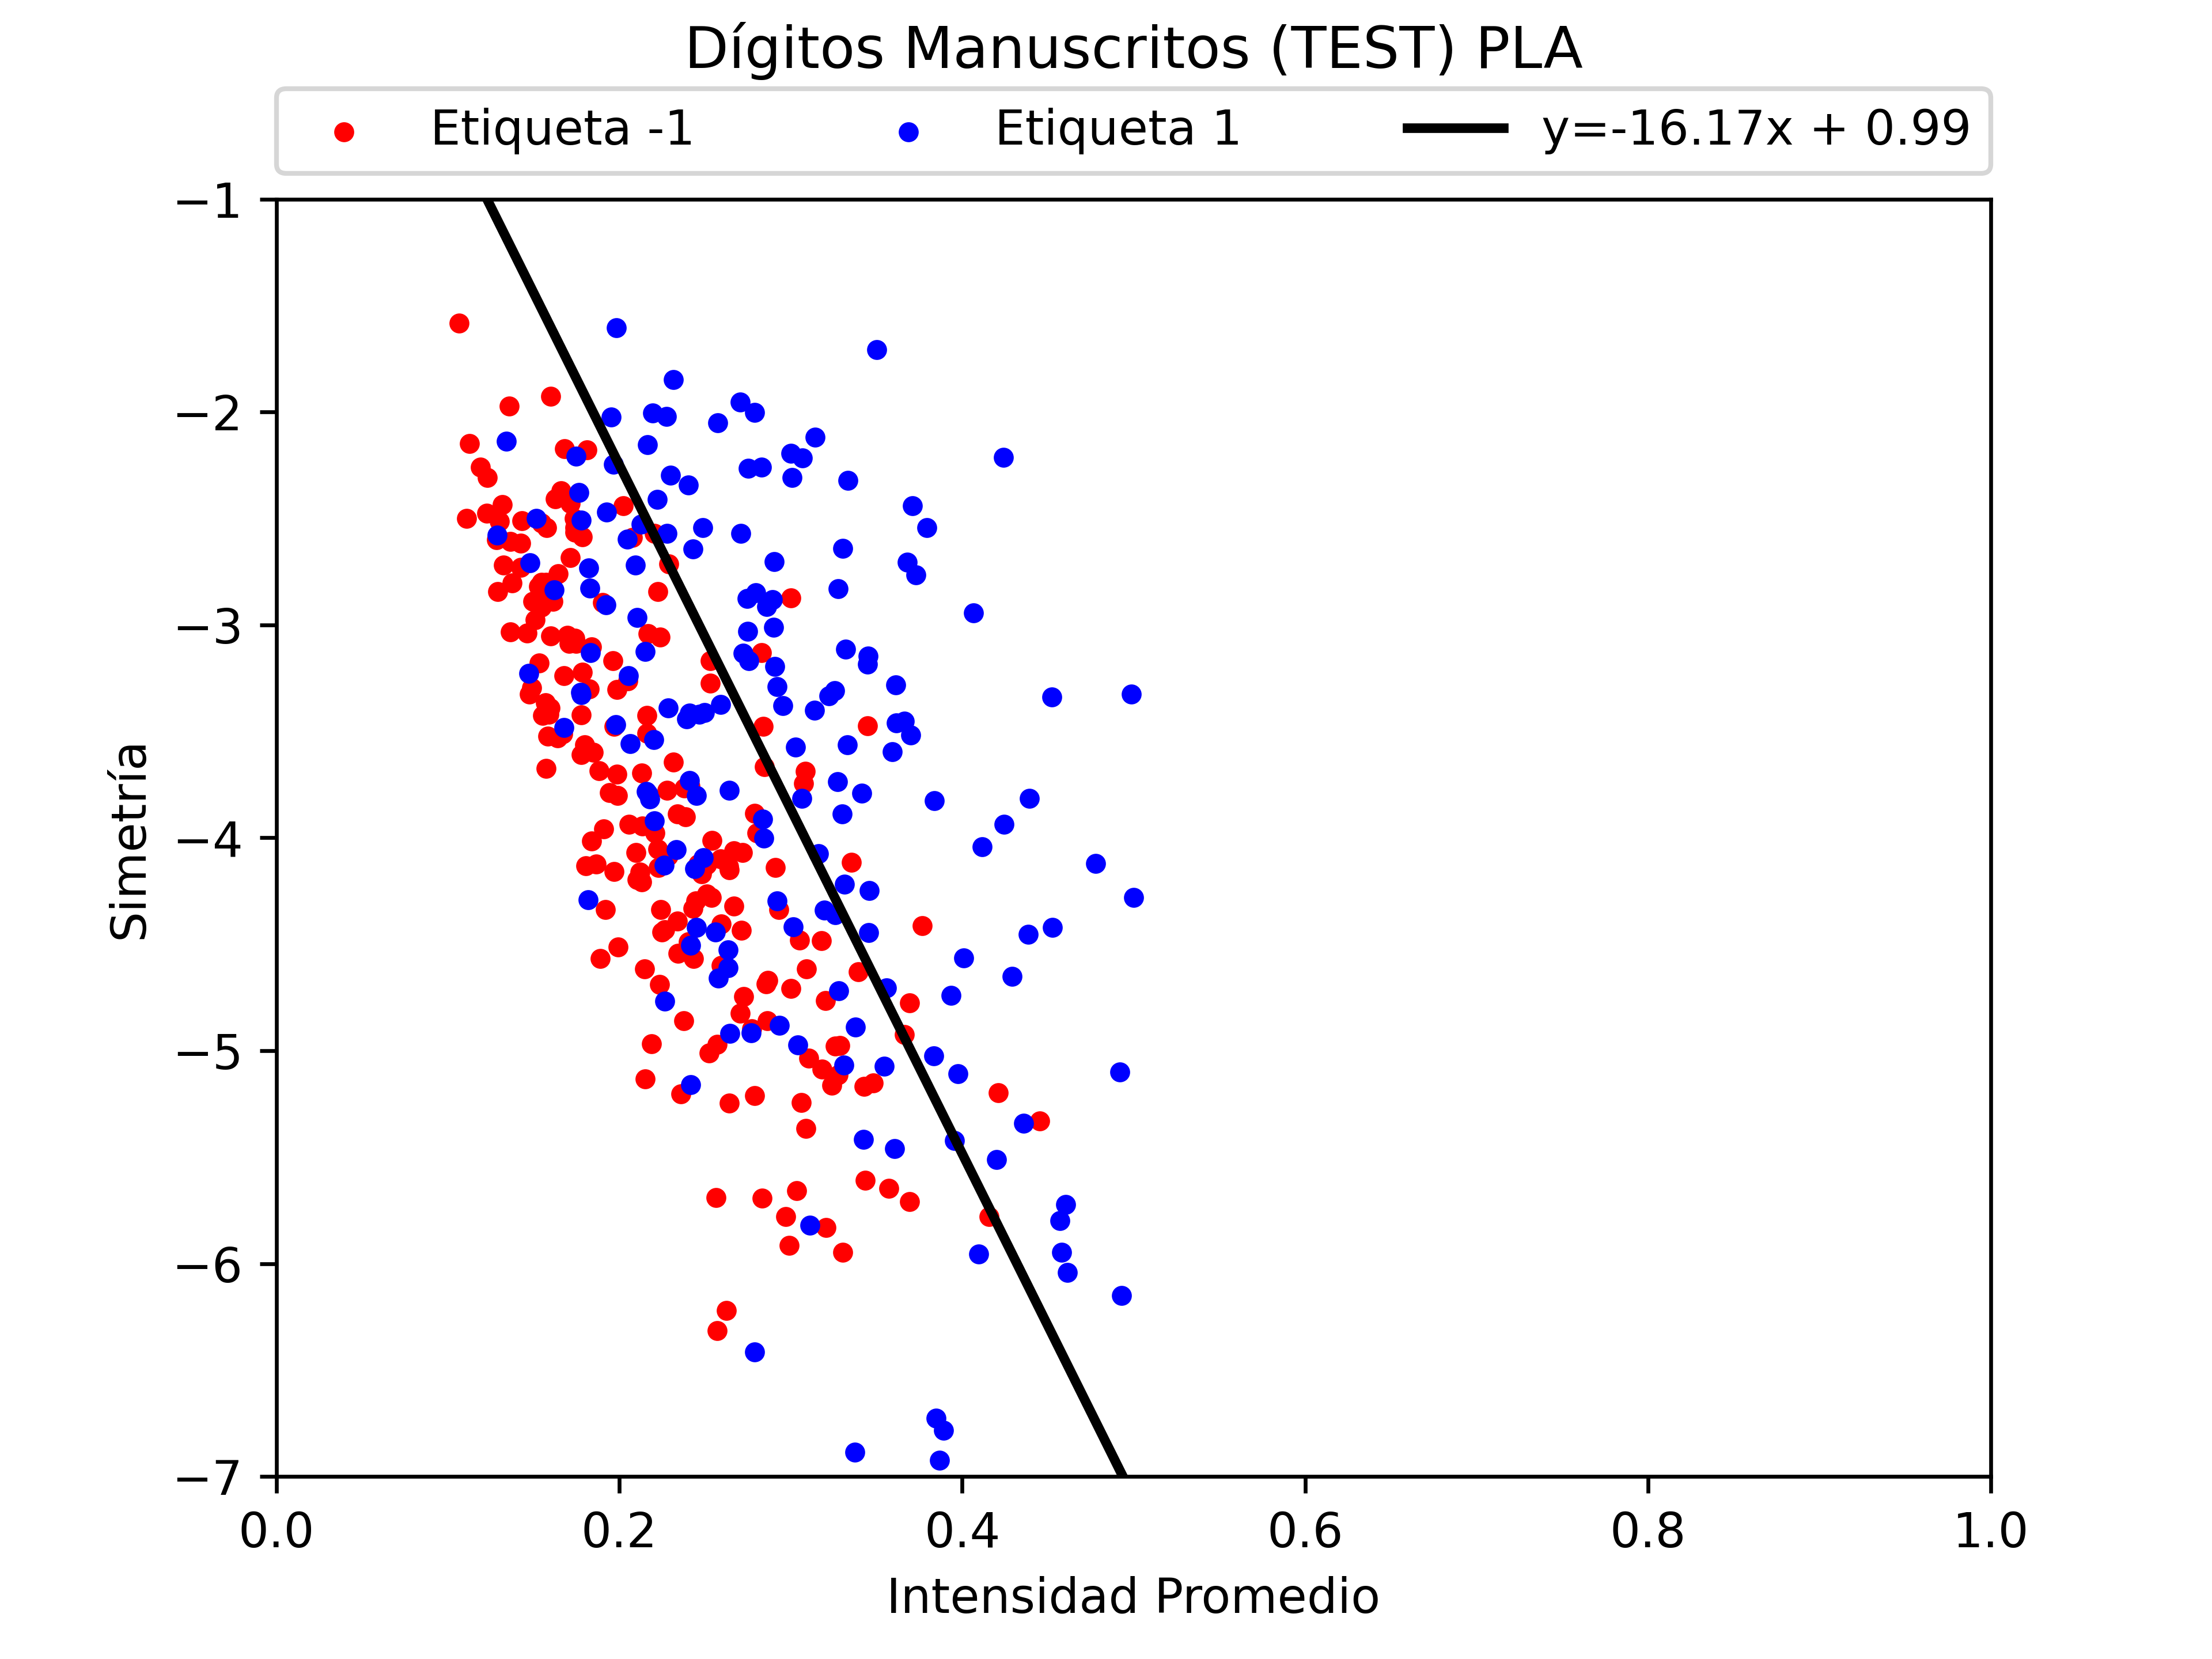
\includegraphics[width=0.9\textwidth]{Figure_24}
      \subcaption{Datos de test}
    \end{minipage}
    \label{fig:dummy66}
\end{figure}

\begin{figure}[H]
    \caption{RL inicializado con $w_{lin}$ \medskip}
    \begin{minipage}[b]{.5\linewidth}
      \centering
      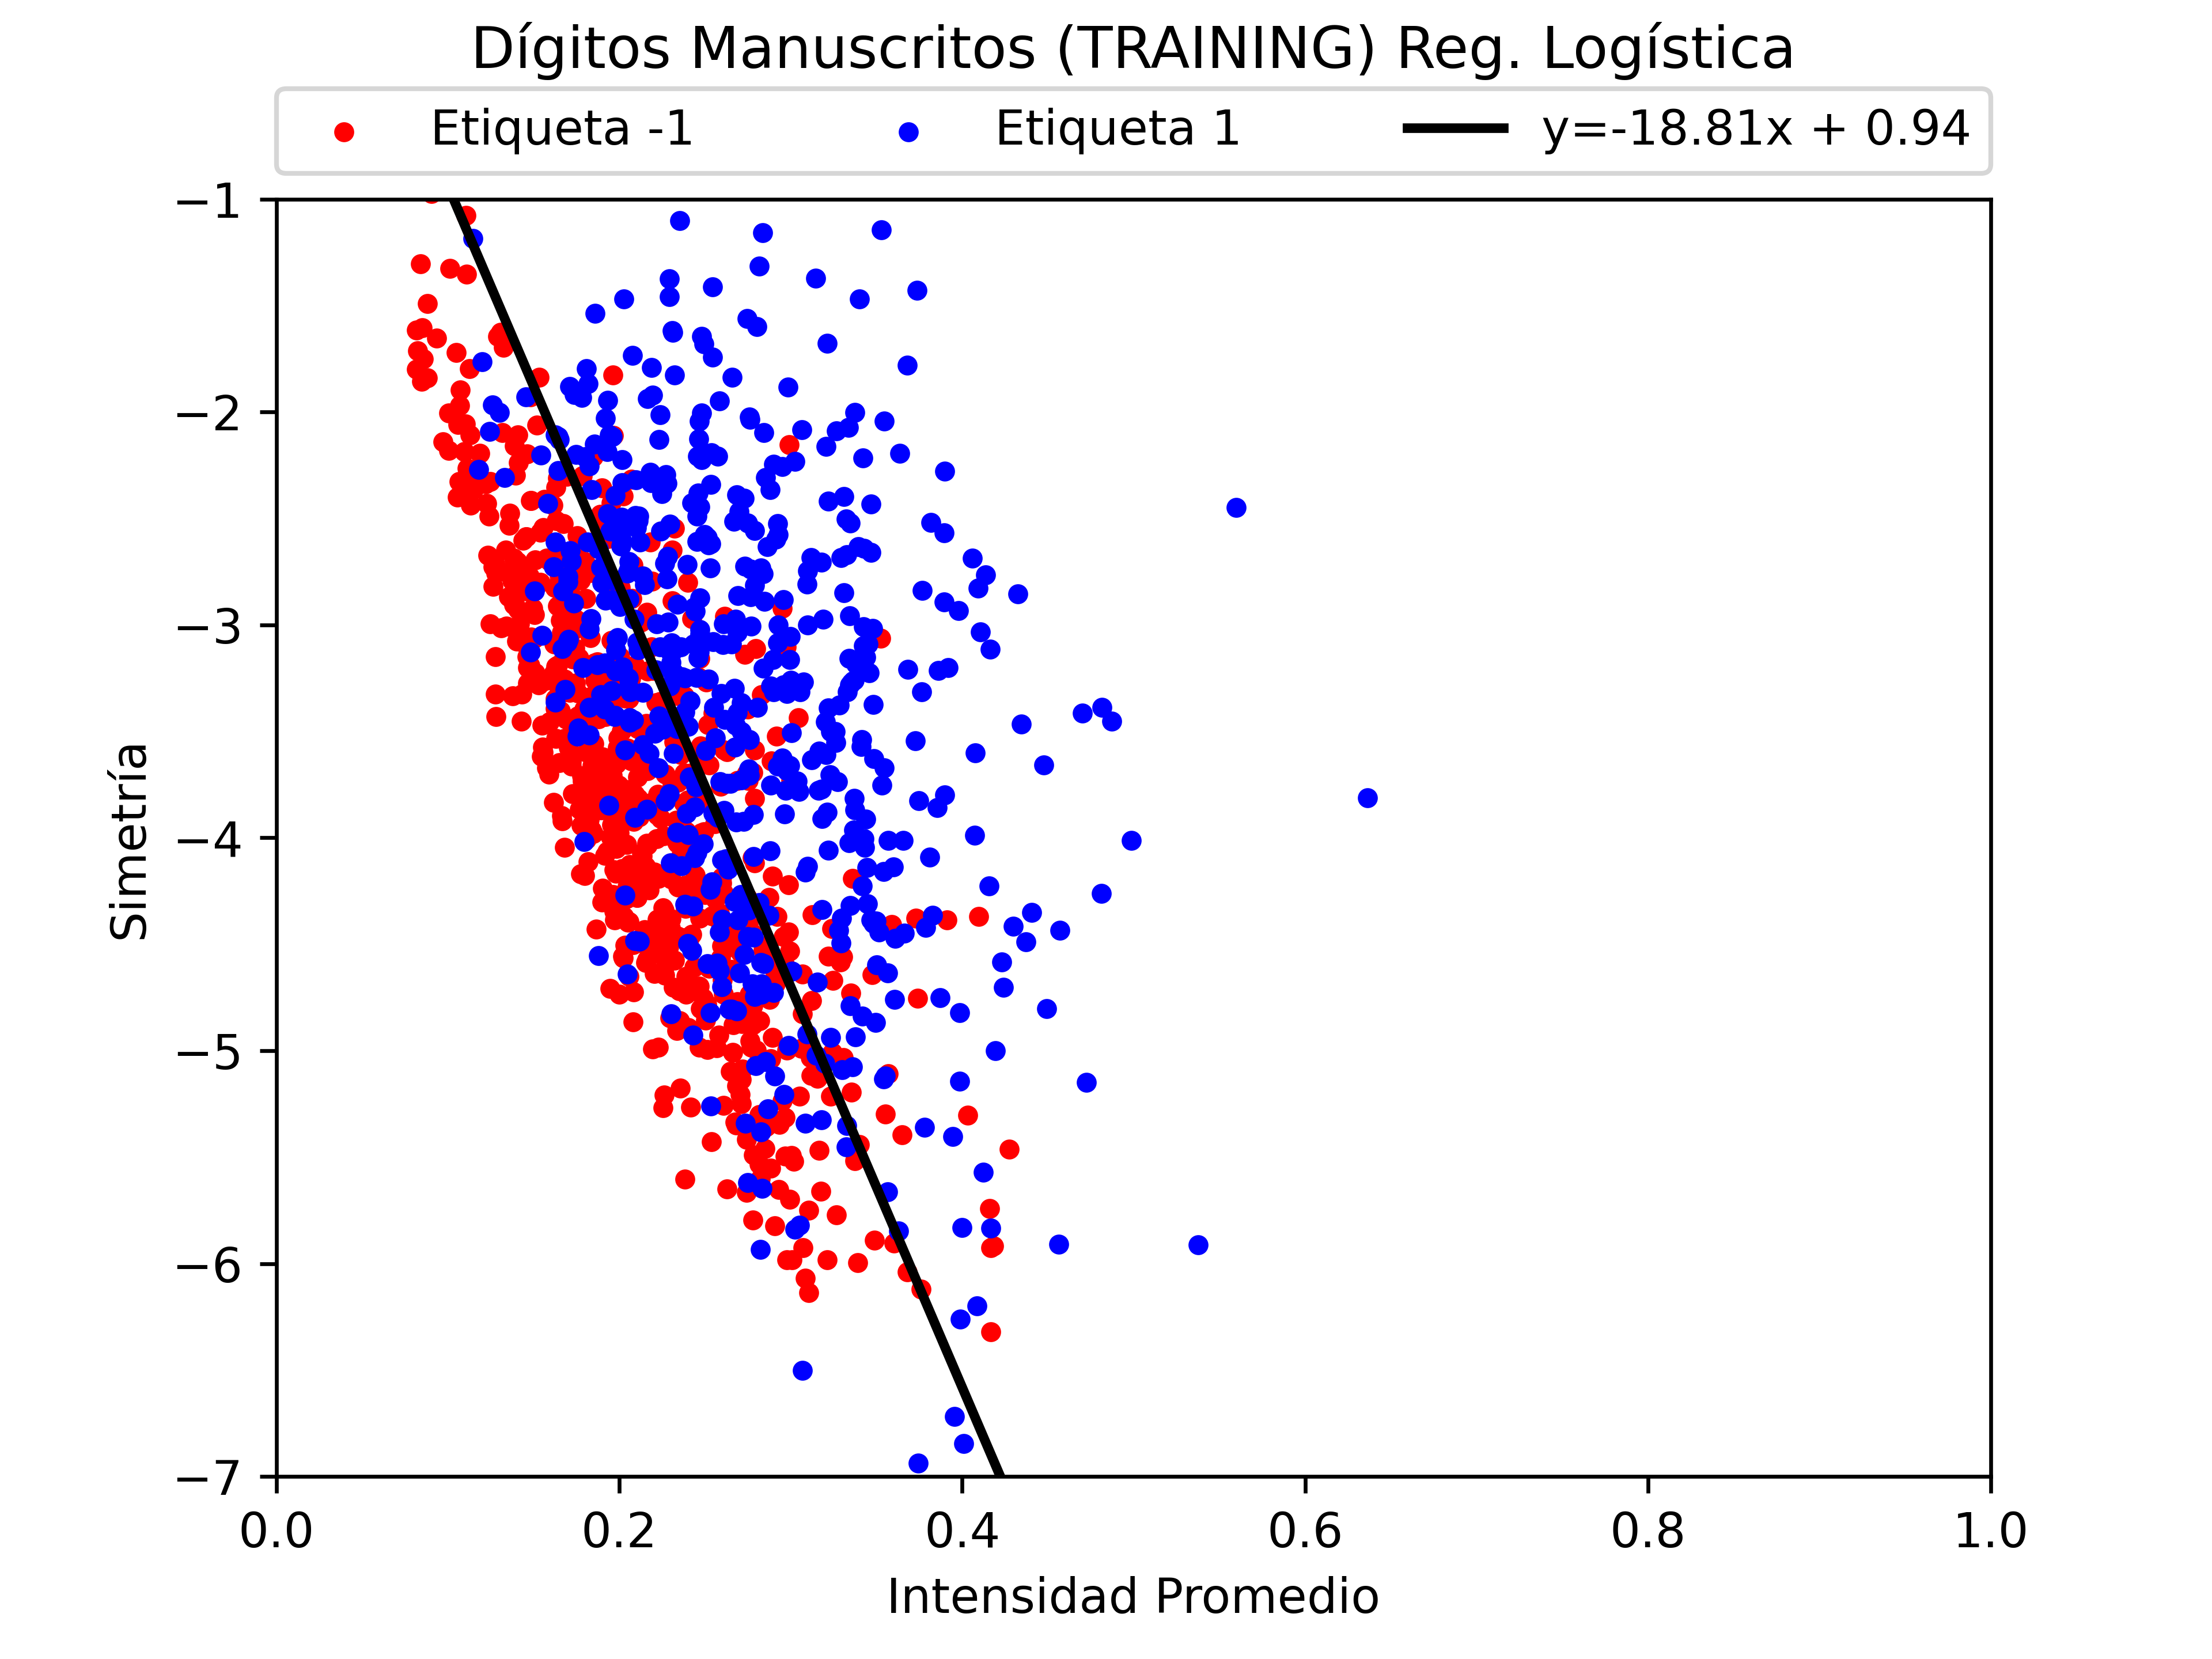
\includegraphics[width=0.9\textwidth]{Figure_25}
      \subcaption{Datos de entrenamiento} \label{subfig-5:dummy67}
    \end{minipage}
    \hfill \hfill
    \begin{minipage}[b]{.5\linewidth}
      \centering
      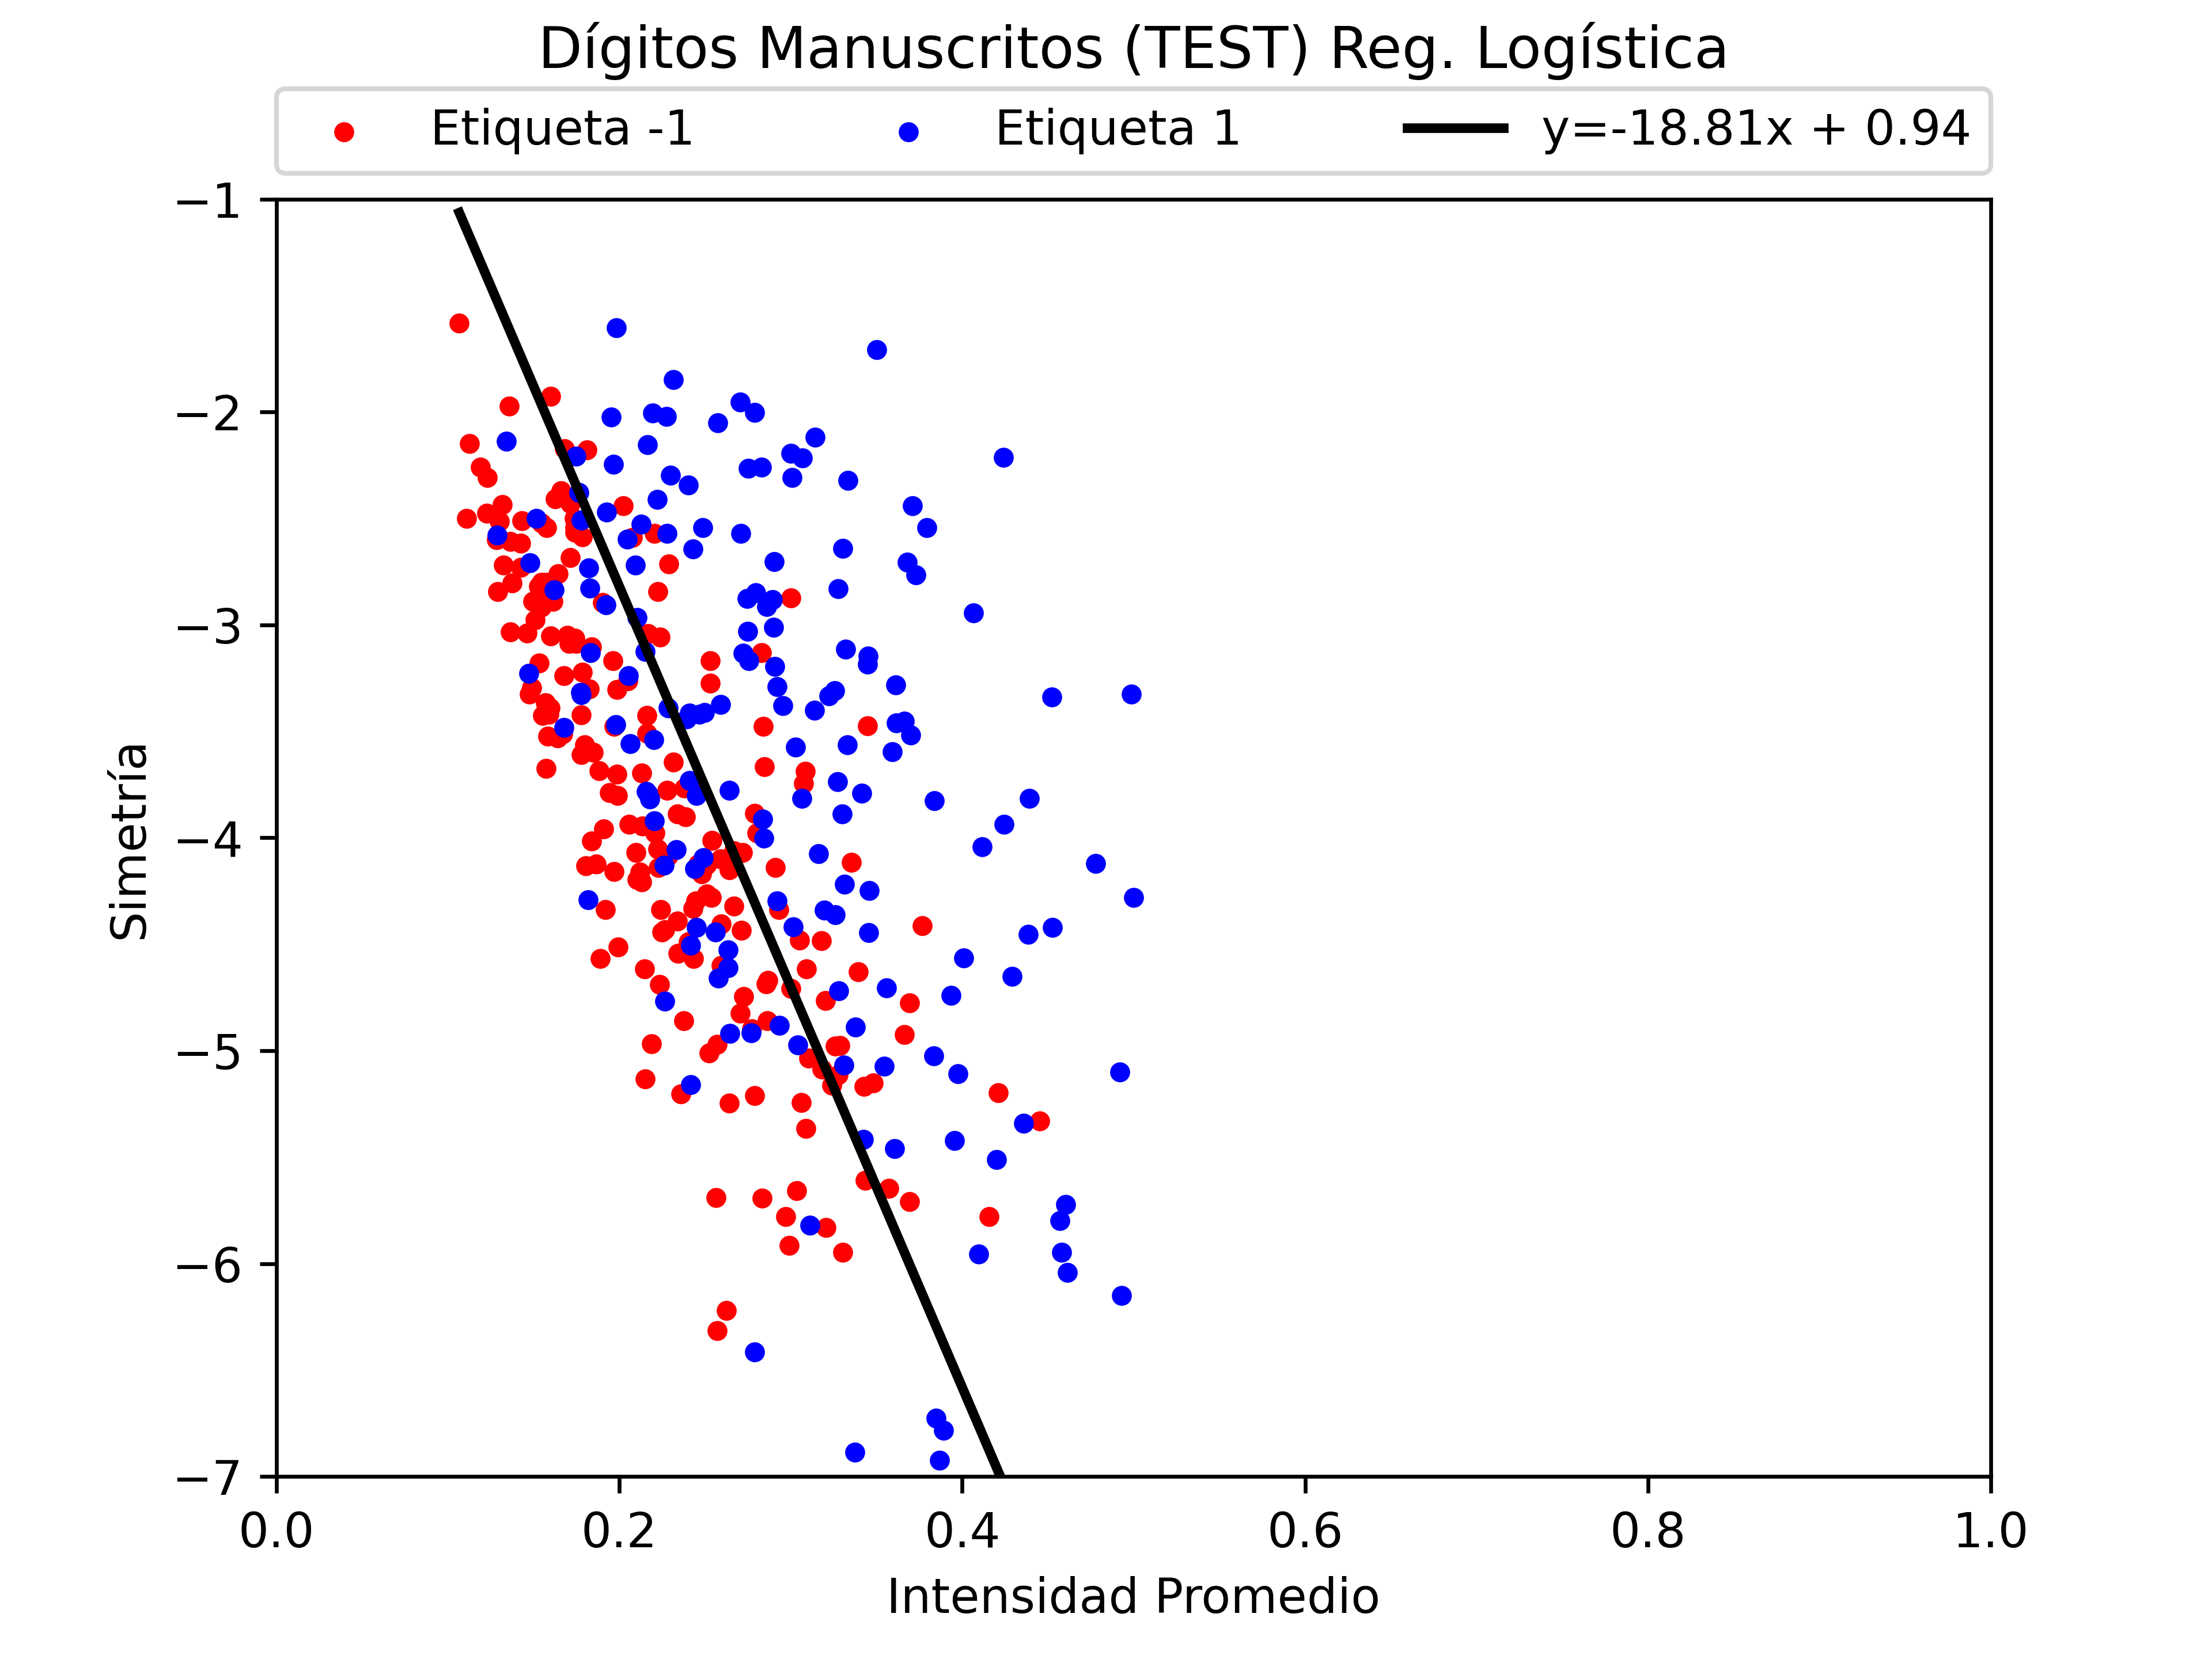
\includegraphics[width=0.9\textwidth]{Figure_26}
      \subcaption{Datos de test}
    \end{minipage}
    \label{fig:dummy67}
\end{figure}


\begin{figure}[H]
    \caption{PLA-POCKET inicializado con $w_{lin}$ \medskip}
    \begin{minipage}[b]{.5\linewidth}
      \centering
      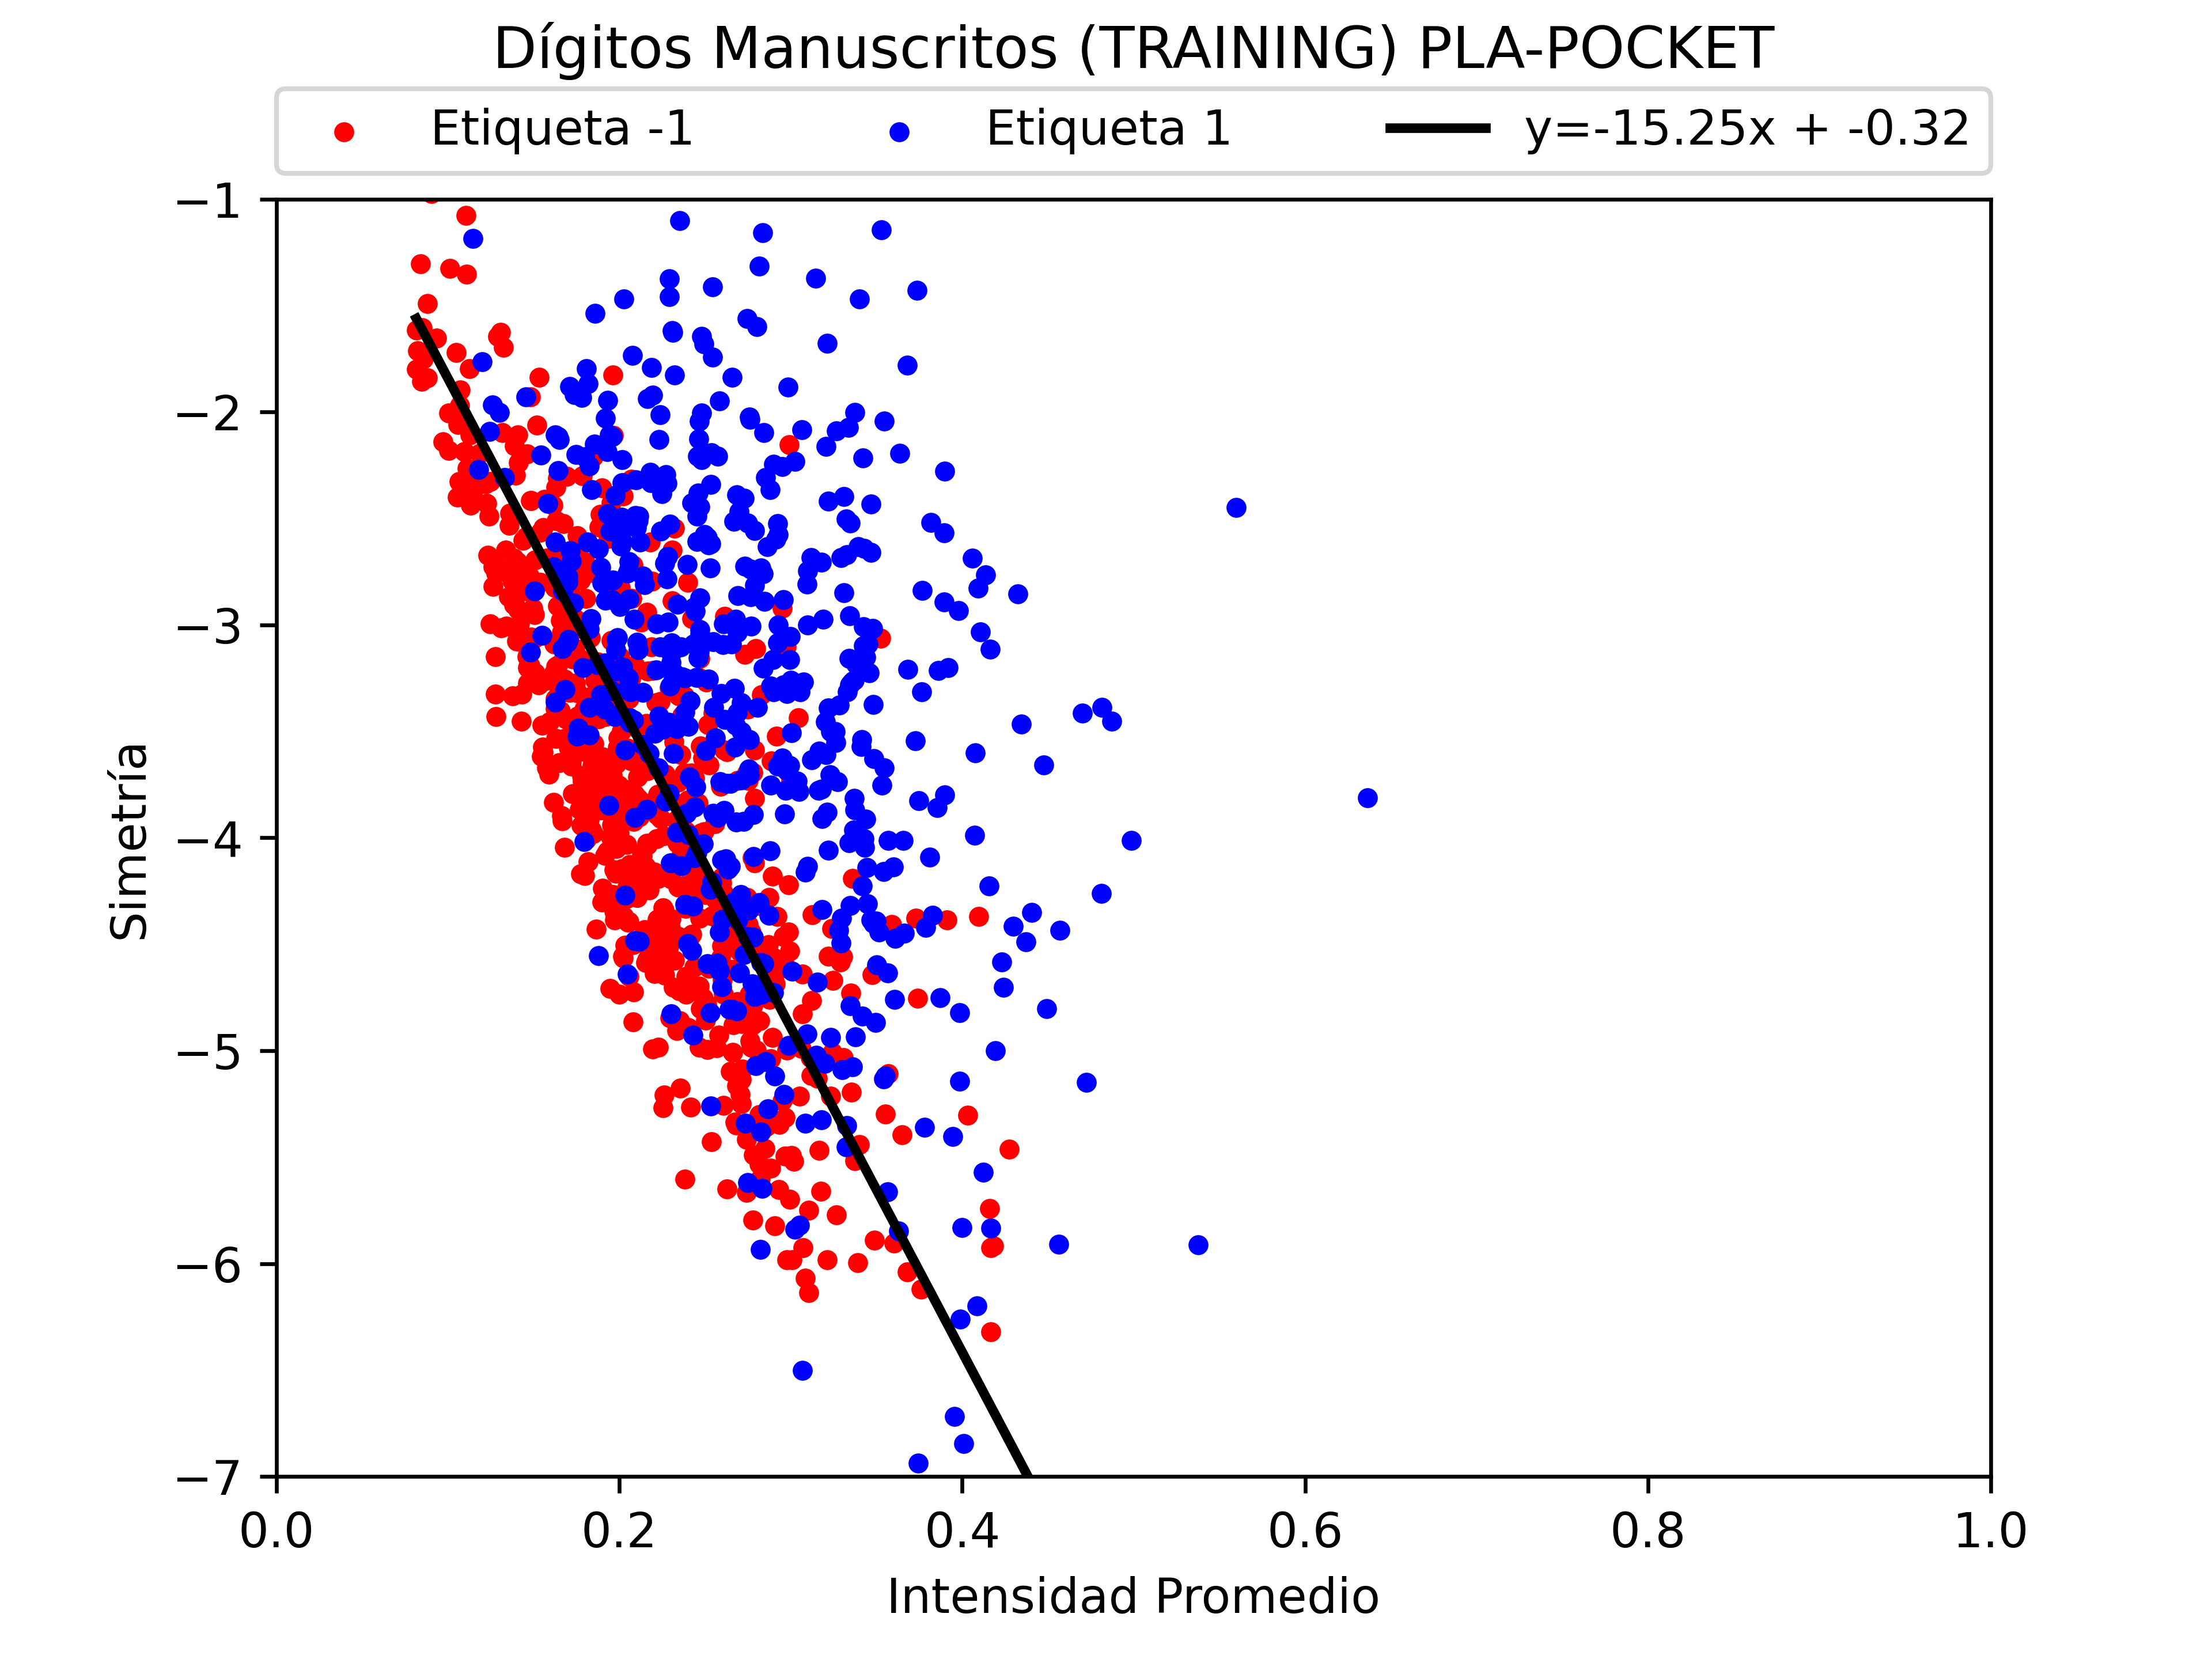
\includegraphics[width=0.9\textwidth]{Figure_27}
      \subcaption{Datos de entrenamiento} \label{subfig-5:dummy68}
    \end{minipage}
    \hfill \hfill
    \begin{minipage}[b]{.5\linewidth}
      \centering
      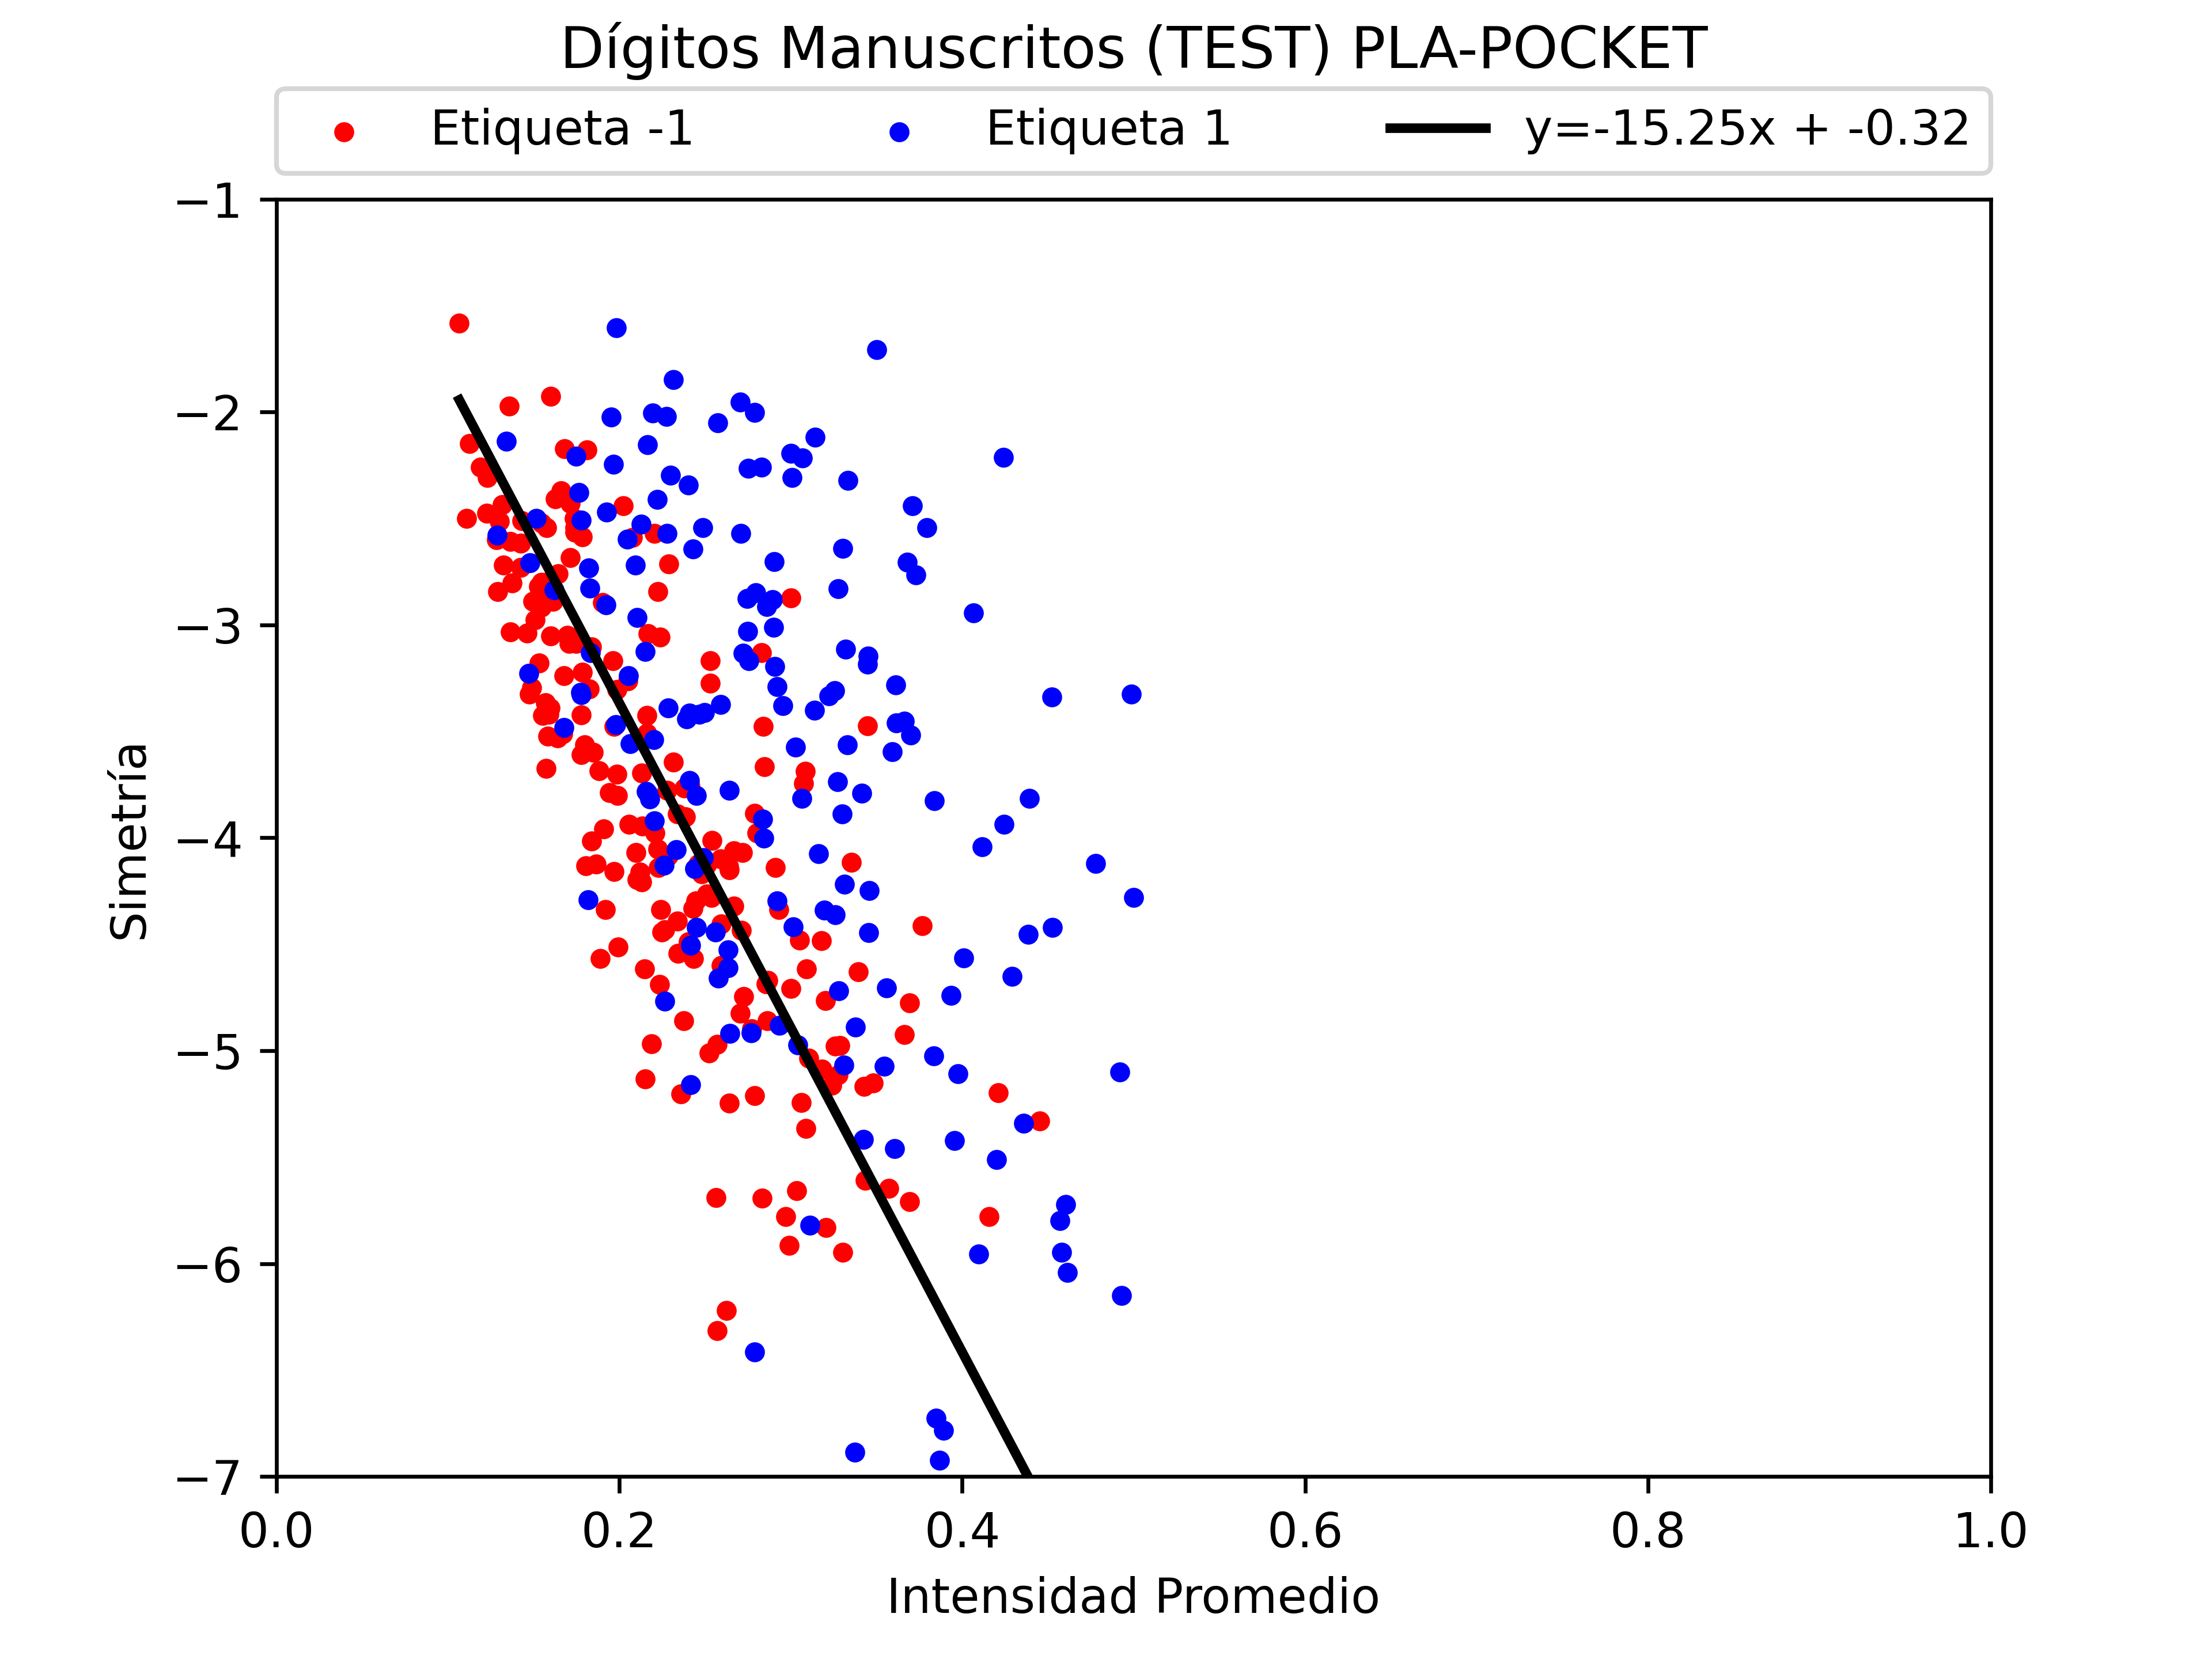
\includegraphics[width=0.9\textwidth]{Figure_28}
      \subcaption{Datos de test}
    \end{minipage}
    \label{fig:dummy68}
\end{figure}

\begin{table}[H]
    \centering
    \begin{tabular}{llll} \toprule
        Algoritmo & $E_{in}$ & $E_{test}$ & Iteraciones \\ \midrule
        PLA & $0.252$ & $0.251$ & $1000$ \\
        RL & $0.465$ & $0.532$ & $588$ \\
        PLA-POCKET & $0.246$ & $0.322$ & $2$ \\ \bottomrule
    \end{tabular}
    \caption{Comparación de modelos lineales iterativos inicializados con $w_{lin}$}
\end{table}

\subsection{Obtener cotas sobre el verdadero valor de $E_{out}$ para los 4 métodos}

\textbf{Calcúlense dos cotas: una basada en $E_{in}$ y otra basada en $E_{test}$.}
\textbf{Usar una tolerancia $\delta=0.05$.}
\textbf{¿Que cota es mejor? Justifique la respuesta.}

